% Task C06
% Source volume: upper
% Physical scan pages: 174--201
% Printed book pages: 157--184
% Transcribe only source content; omit running headers, footers, and printed page numbers.
\chapter{导数与微分}

这是进入微分学的第一章。本章含有四节。在 §6.1 中介绍导数概念、基本的求导公式和计算，§6.2 介绍高阶导数及其他求导法则，一阶微分的概念在 §6.3 中讨论，最后一节为学习要点和两组参考题。

\section{导数及其计算}

\subsection{内容提要}

这里的要点为
\begin{enumerate}
  \item 导数就是变量的变化率。它在几何上来源于如何定义一般曲线的切线，而在运动学上则与中学物理中的瞬时速度的定义方式完全相同。
  \item 从导数的定义可以看出，计算导数就是要求 $\frac{0}{0}$ 型的不定式的函数极限。这也就是在学习微分学之前先要学习极限理论的理由之一。§4.3 的两个重要极限以及许多例题都与此直接相关。
  \item 函数在某一个点是否可导，只与该函数在这点附近的性态有关。因此与函数的极限和连续性类似，函数的可导性是一种局部性概念。
  \item 函数在一点可导，则一定在该点连续。反之未必成立。
  \item 除了导数的几何意义之外，还要知道单侧导数的几何意义，以及在某一点的导数或单侧导数为无穷大时的几何意义。
  \item 导函数的概念。这直接导致高阶导数的概念。
  \item 导数的计算。初等函数的导函数仍是初等函数。这里的计算可以用求导公式按部就班地进行。对于分段定义的函数，在特殊点上要从导数定义出发直接计算。
  \item 复合函数求导的链式法则是导数计算中的基本工具。
  \item 对隐函数和用参数方程定义的函数的导数计算所涉及的理论问题将在以后学习，本章着重于学习用求导法则进行计算。
\end{enumerate}

初等函数的求导公式在数学分析的教科书中都有，本书不再重复。请初学者注意：求导数是数学分析中最基本的一项计算，而这必须通过做教科书中的大量导数计算题才能学会。否则连基本公式都记不住，还有什么技能可谈。

\subsection{思考题}

\begin{xthought}[1]
设 $f\in C(a,b)$，又在点 $x_0\in(a,b)$ 处可导。在 $x\ne x_0$ 时定义函数
  \[
    g(x)=\frac{f(x)-f(x_0)}{x-x_0}.
  \]
  问：如何在 $x_0$ 处补充定义 $g(x)$ 才能使得 $g\in C(a,b)$？
\end{xthought}
\begin{xsolution}
应补充定义
\[
  g(x_0)=f'(x_0).
\]
事实上，由 $f$ 在 $x_0$ 处可导，
\[
  \lim_{x\to x_0}\frac{f(x)-f(x_0)}{x-x_0}=f'(x_0),
\]
故如此定义后 $g$ 在 $x_0$ 处连续；而在 $x\ne x_0$ 处，$g$ 是连续函数的商，分母不为零，所以 $g$ 连续。因此 $g\in C(a,b)$。
\end{xsolution}


\begin{xthought}[2]
说明 $f'_+(x_0)$ 和 $f'(x_0^+)$ 的不同意义，并举出它们取不同数值的例子。
\end{xthought}
\begin{xsolution}
$f'_+(x_0)$ 是 $f$ 在点 $x_0$ 的右导数：
\[
  f'_+(x_0)=\lim_{h\to0^+}\frac{f(x_0+h)-f(x_0)}h.
\]
而 $f'(x_0^+)$ 表示导函数 $f'$ 在 $x_0$ 的右极限：
\[
  f'(x_0^+)=\lim_{x\to x_0^+}f'(x),
\]
它要求 $f$ 在 $x_0$ 右侧邻域内可导。

二者是不同概念。例如令
\[
  f(x)=
  \begin{cases}
    x^2\sin\dfrac1x,&x\ne0,\\
    0,&x=0.
  \end{cases}
\]
则 $f'_+(0)=0$，但
\[
  f'(x)=2x\sin\frac1x-\cos\frac1x\qquad(x\ne0),
\]
所以 $f'(0^+)$ 不存在。

若 $f'_+(x_0)$ 与有限极限 $f'(x_0^+)$ 都存在，则二者不能取不同的有限数值；在通常的单侧导数极限定理条件下必有 $f'_+(x_0)=f'(x_0^+)$。因此本题所要强调的是“概念不同”，而不是在二者都存在时可以有两个不同的有限值。
\end{xsolution}


\begin{xthought}[3]
$f'(x_0)$ 和 $(f(x_0))'$ 有无区别？为什么？
\end{xthought}
\begin{xsolution}
有区别。$f'(x_0)$ 是函数 $f$ 在点 $x_0$ 的导数；而 $f(x_0)$ 是一个固定常数。若把 $(f(x_0))'$ 理解为对变量 $x$ 求导，则其值为 $0$。因此一般有
\[
  (f(x_0))'=0,
\]
而 $f'(x_0)$ 未必为零。
\end{xsolution}


\begin{xthought}[4]
验证下列三个函数 $f(x)=\sin^2x$，$g(x)=-\cos^2x$，$h(x)=-\frac12\cos2x$ 的导函数均相等。为什么相等？
\end{xthought}
\begin{xsolution}
逐一求导：
\[
  (\sin^2x)'=2\sin x\cos x=\sin2x,
\]
\[
  (-\cos^2x)'=2\sin x\cos x=\sin2x,
\]
以及
\[
  \left(-\frac12\cos2x\right)'=\sin2x.
\]
三者导函数相同。原因也可由恒等式看出：
\[
  \sin^2x=-\frac12\cos2x+\frac12,
  \qquad
  -\cos^2x=-\frac12\cos2x-\frac12.
\]
三函数彼此只相差常数，而常数的导数为零。
\end{xsolution}


\begin{xthought}[5]
若 $f'(x_0)$ 存在，求
  \[
    \lim_{\Delta x\to0}\frac{f(x_0-\Delta x)-f(x_0)}{\Delta x}.
  \]
\end{xthought}
\begin{xsolution}
令 $h=-\Delta x$，则当 $\Delta x\to0$ 时 $h\to0$，且
\[
  \frac{f(x_0-\Delta x)-f(x_0)}{\Delta x}
  =-\frac{f(x_0+h)-f(x_0)}h.
\]
故
\[
  \lim_{\Delta x\to0}\frac{f(x_0-\Delta x)-f(x_0)}{\Delta x}
  =-f'(x_0).
\]
\end{xsolution}


\begin{xthought}[6]
若 $[f(x)]'=[f^2(x)]'$，证明：或者 $f(1)=1$，或者 $f'(1)=0$。
\end{xthought}
\begin{xsolution}
由题设
\[
  [f(x^2)]'=[f^2(x)]'.
\]
按复合函数求导法则与乘方求导法则，
\[
  2x f'(x^2)=2f(x)f'(x).
\]
令 $x=1$，得到
\[
  2f'(1)=2f(1)f'(1),
\]
即
\[
  [1-f(1)]f'(1)=0.
\]
因此必有
\[
  \boxed{f(1)=1\quad\text{或}\quad f'(1)=0}.
\]
\end{xsolution}


\begin{xthought}[7]
\begin{enumerate}[label=(\arabic*)]
    \item 在圆面积公式 $S(r)=\pi r^2$ 和圆周长公式 $l(r)=2\pi r$ 之间有微分学的关系 $S'(r)=l(r)$，请作出解释；
    \item 同样，在球体积公式 $V(r)=\frac43\pi r^3$ 和球面积公式 $A(r)=4\pi r^2$ 之间有微分学的关系 $V'(r)=A(r)$，请作出解释；
    \item 能否在所知的初等几何计算公式中再找出类似的微分学联系？
  \end{enumerate}
\end{xthought}
\begin{xsolution}
\begin{enumerate}[label=(\arabic*)]
  \item 半径由 $r$ 增加到 $r+\Delta r$ 时，圆面积增量为
  \[
    \Delta S=\pi(r+\Delta r)^2-\pi r^2
    =2\pi r\,\Delta r+\pi(\Delta r)^2.
  \]
  其线性主部为 $2\pi r\,\Delta r=l(r)\Delta r$，因此
  \[
    S'(r)=2\pi r=l(r).
  \]
  几何上，薄圆环的面积在一阶近似下等于“圆周长 $\times$ 厚度”。

  \item 同理，
  \[
    \Delta V=\frac43\pi(r+\Delta r)^3-\frac43\pi r^3
    =4\pi r^2\Delta r+\bigO((\Delta r)^2),
  \]
  所以
  \[
    V'(r)=4\pi r^2=A(r).
  \]
  即薄球壳体积的一阶主部等于“球面积 $\times$ 厚度”。

  \item 例如固定高 $h$ 的圆柱体
  \[
    V(r)=\pi r^2h,
  \]
  对半径求导得到
  \[
    V'(r)=2\pi rh,
  \]
  正好等于圆柱的侧面积。又如矩形面积 $A(x)=xh$ 对边长 $x$ 求导得 $A'(x)=h$，即等于随 $x$ 移动的那条边的长度。
\end{enumerate}
\end{xsolution}


\begin{xthought}[8]
设 $f(x)$ 在 $(a,b)$ 上可导。
  \begin{enumerate}[label=(\arabic*)]
    \item 若 $\lim_{x\to a^+}f(x)=\infty$，是否可以推出 $\lim_{x\to a^+}f'(x)=\infty$？
    \item 若 $\lim_{x\to a^+}f'(x)=\infty$，是否可以推出 $\lim_{x\to a^+}f(x)=\infty$？
  \end{enumerate}
\end{xthought}
\begin{xsolution}
两问的答案都是否定的。
\begin{enumerate}[label=(\arabic*)]
  \item 取
  \[
    f(x)=\frac1{x-a}\qquad(x>a).
  \]
  则 $x\to a^+$ 时 $f(x)\to+\infty$，但
  \[
    f'(x)=-\frac1{(x-a)^2}\to-\infty,
  \]
  并非趋于 $+\infty$。

  \item 取
  \[
    f(x)=\sqrt{x-a}\qquad(x>a).
  \]
  则
  \[
    f'(x)=\frac1{2\sqrt{x-a}}\to+\infty,
  \]
  但 $f(x)\to0$，并不趋于 $+\infty$。
\end{enumerate}
\end{xsolution}


\begin{xthought}[9]
判断下列命题的真假，并说明理由：
  \begin{enumerate}[label=(\arabic*)]
    \item 若 $f$ 在 $x=0$ 可导，且 $f(0)=0$，则 $f'(0)=0$；反之也成立；
    \item 若 $f$ 在 $x_0$ 可导，且在某 $O(x_0)$ 上 $f(x)>0$，则 $f'(x_0)>0$；
    \item 若 $f$ 为 $(-1,1)$ 上的偶函数，于 $x=0$ 处可导，则 $f'(0)=0$；
    \item 若 $f$ 为 $(-1,1)$ 上的奇函数，于 $x=0$ 处可导，则 $f'(0)=0$；
    \item 若 $f$ 在 $x_0$ 可导，则 $\abs{f}$ 也在 $x_0$ 处可导；反之也成立；
    \item 若存在极限
    \[
      \lim_{\Delta x\to0}\frac{f(x_0+\Delta x)-f(x_0-\Delta x)}{\Delta x},
    \]
    则 $f(x)$ 于 $x_0$ 处可导；反之也成立。
  \end{enumerate}
\end{xthought}
\begin{xsolution}
\begin{enumerate}[label=(\arabic*)]
  \item 假。取 $f(x)=x$，则 $f(0)=0$ 而 $f'(0)=1$。反过来也假，例如 $f(x)=x^2+1$ 有 $f'(0)=0$ 而 $f(0)=1$。

  \item 假。取 $x_0=0$，$f(x)=1-x$。在 $0$ 的充分小邻域内 $f(x)>0$，但 $f'(0)=-1<0$。

  \item 真。偶性给出 $f(h)=f(-h)$，故
  \[
    f'(0)=\lim_{h\to0}\frac{f(h)-f(0)}h
    =-\lim_{h\to0}\frac{f(-h)-f(0)}{-h}=-f'(0),
  \]
  从而 $f'(0)=0$。

  \item 假。$f(x)=x$ 是奇函数，但 $f'(0)=1$。

  \item 两个方向都不成立。正向反例为 $f(x)=x$、$x_0=0$：$f$ 可导，但 $\abs{f(x)}=\abs{x}$ 在 $0$ 不可导。反向可取
  \[
    f(x)=
    \begin{cases}
      1,&x\in\QQ,\\
      -1,&x\notin\QQ.
    \end{cases}
  \]
  则 $\abs{f(x)}\equiv1$ 处处可导，而 $f$ 处处不连续，因而处处不可导。

  \item “存在所给对称差商极限 $\Rightarrow$ 可导”是假。取 $f(x)=\abs{x}$，$x_0=0$，有
  \[
    \frac{f(h)-f(-h)}h=0,
  \]
  但 $f$ 在 $0$ 不可导。反之若 $f$ 在 $x_0$ 可导，则
  \begin{align*}
    \frac{f(x_0+h)-f(x_0-h)}h
    &=\frac{f(x_0+h)-f(x_0)}h
      +\frac{f(x_0)-f(x_0-h)}h\\
    &\longrightarrow f'(x_0)+f'(x_0)=2f'(x_0),
  \end{align*}
  因而反向成立。
\end{enumerate}
\end{xsolution}


\begin{xthought}[10]
\begin{enumerate}[label=(\arabic*)]
    \item 如果 $f(x)$ 在点 $x_0$ 处既左连续，又右连续，问 $f(x)$ 在 $x_0$ 处是否连续？
    \item 如果 $f(x)$ 在点 $x_0$ 处既左侧可导，又右侧可导，问 $f(x)$ 在 $x_0$ 处是否可导？为什么？
  \end{enumerate}
\end{xthought}
\begin{xsolution}
\begin{enumerate}[label=(\arabic*)]
  \item 是。左连续与右连续分别给出
  \[
    \lim_{x\to x_0^-}f(x)=f(x_0),
    \qquad
    \lim_{x\to x_0^+}f(x)=f(x_0),
  \]
  两个单侧极限相等，因此 $f$ 在 $x_0$ 连续。

  \item 未必。只有当左导数与右导数存在且相等时才可导。反例为 $f(x)=\abs{x}$ 在 $0$ 处：
  \[
    f'_-(0)=-1,\qquad f'_+(0)=1,
  \]
  两个单侧导数都存在，但不相等，所以 $f'(0)$ 不存在。
\end{enumerate}
\end{xsolution}


\subsection{例题}

以下第一个例题的内容是联系导数与连续的基本结果。

\begin{xexample}[6.1.1]
证明：函数在某点可导，则在该点一定连续。
\end{xexample}
\begin{xproof}
证 1\quad 设函数 $y=f(x)$ 于点 $x_0$ 处可导。根据定义，存在极限
\[
  \lim_{\Delta x\to0}\frac{\Delta y}{\Delta x}=f'(x_0).
\]
因此有
\[
  \frac{\Delta y}{\Delta x}=f'(x_0)+\littleo(1)\quad(\Delta x\to0).
\]
两边乘以 $\Delta x$，得到
\begin{equation}
  \Delta y=f'(x_0)\Delta x+\littleo(\Delta x)\quad(\Delta x\to0).
  \tag{6.1}
  \label{eq:6.1}
\end{equation}
由于 $\Delta x=x-x_0,\Delta y=y-y_0=f(x)-f(x_0)$，上式可以重写为
\[
  f(x)=f(x_0)+f'(x_0)(x-x_0)+\littleo(x-x_0)\quad(x\to x_0).
\]
令 $x\to x_0$，就得到 $\lim_{x\to x_0}f(x)=f(x_0)$。
\end{xproof}

\begin{xremark}
称 (6.1) 为无穷小增量公式。它是微分学中的主要工具之一。
\end{xremark}

\begin{xproof}
证 2\quad 将函数 $y=f(x)$ 的因变量 $y$ 的增量 $\Delta y$ 写成（$\Delta x\ne0$）
\[
  \Delta y=\frac{\Delta y}{\Delta x}\cdot\Delta x.
\]
由于右边的差商当 $\Delta x\to0$ 时有极限，第二个因子是无穷小量，因此就得到
\[
  \Delta y=\littleo(1)\quad(\Delta x\to0).
\]
这就是说当 $x\to x_0$ 时 $f(x)\to f(x_0)$，即 $f$ 在 $x_0$ 处连续。
\end{xproof}

\begin{xproof}
证 3\quad 直接用连续性的 $\varepsilon$-$\delta$ 定义来进行证明。由于存在极限
\[
  \lim_{x\to x_0}\frac{f(x)-f(x_0)}{x-x_0}=f'(x_0),
\]
应用局部有界性定理，存在 $M>0,\eta>0$，使得当 $0<\abs{x-x_0}<\eta$ 时，成立
\[
  \abs{\frac{f(x)-f(x_0)}{x-x_0}}<M.
\]
对给定的 $\varepsilon>0$，取
\[
  \delta=\min\left\{\eta,\frac{\varepsilon}{M}\right\}.
\]
则当 $0<\abs{x-x_0}<\delta$ 时，成立
\[
  \abs{f(x)-f(x_0)}
  =\abs{\frac{f(x)-f(x_0)}{x-x_0}}\cdot\abs{x-x_0}
  <M\abs{x-x_0}\le\varepsilon.
\]
这样就证明了 $f$ 在 $x_0$ 处连续。
\end{xproof}

\begin{xremark}
与这个基本结论有关的其他内容有：(1) 若 $f(x)$ 在点 $x_0$ 存在某个单侧导数，则 $f(x)$ 在点 $x_0$ 具有相应的单侧连续性；(2) 若 $f(x)$ 在点 $x_0$ 存在两个单侧导数（不论它们是否相等），则 $f(x)$ 在点 $x_0$ 处连续。（典型例子为 $f(x)=\abs{x},x_0=0$。）
\end{xremark}

\begin{xexample}[6.1.2]
举例说明函数在某点可导，但在这点外的每个点上可以不连续。
\end{xexample}
\begin{xsolution}
定义函数 $f$ 如下：
\[
  f(x)=
  \begin{cases}
    x^2, & x\text{ 是有理数},\\
    0,   & x\text{ 是无理数}.
  \end{cases}
\]
则在 $x=0$ 处 $f'(0)=0$，当然函数于该点连续。但在任何 $x\ne0$ 处函数 $f$ 均有第二类间断点（证明细节请读者完成）。
\end{xsolution}

若 $y=f(x)$ 在点 $x_0$ 处可导，则曲线 $y=f(x)$ 在点 $(x_0,f(x_0))$ 处有切线
\[
  l(x)=f(x_0)+f'(x_0)(x-x_0).
\]
下一个例题刻画了这条特殊的直线所具有的局部最优性（见 [17]）。

\begin{xexample}[6.1.3]
设函数 $f(x)$ 在点 $x_0$ 处可导，$l(x)$ 定义如上。对于不等于 $l(x)$ 的其他任何 $L(x)=ax+b$，存在 $\delta>0$，使得当 $0<\abs{x-x_0}<\delta$ 时，成立不等式
\begin{equation}
  \abs{f(x)-l(x)}<\abs{f(x)-L(x)}.
  \tag{6.2}
  \label{eq:6.2}
\end{equation}
\end{xexample}
\begin{xproof}
如图 6.1 所示分两种情况讨论。

\begin{center}
  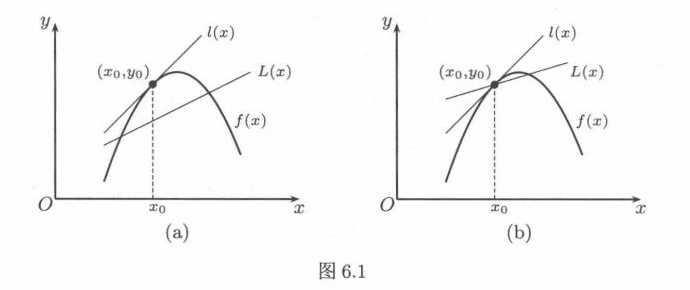
\includegraphics[width=.72\linewidth]{figures/upper/ch06/fig-6-1.png}
\end{center}

(1) $L(x_0)\ne f(x_0)$。几何上这表明直线 $L(x)=ax+b$ 不经过点 $(x_0,y_0)$，其中 $y_0=f(x_0)=l(x_0)$。由于 $L(x_0)\ne y_0$，利用
\[
  \lim_{x\to x_0}\abs{f(x)-l(x)}=\abs{f(x_0)-l(x_0)}=0
  <\abs{f(x_0)-L(x_0)}
  =\lim_{x\to x_0}\abs{f(x)-L(x)}
\]
和连续函数的局部保号性，存在 $\delta>0$，使得当 $\abs{x-x_0}<\delta$ 时，所要的不等式 (6.2) 成立。注意：这时 $x=x_0$ 是允许的。

(2) $L(x_0)=f(x_0)$。几何上这表明直线 $L(x)=ax+b$ 经过点 $(x_0,y_0)$，即有
\[
  L(x_0)=f(x_0)=l(x_0)=ax_0+b.
\]
改写 $L(x)$ 为
\[
  L(x)=a(x-x_0)+f(x_0).
\]
由于 $L(x)\ne l(x)$，所以必有 $a\ne f'(x_0)$。由于导数 $f'(x_0)$ 存在，即有（这就是无穷小增量公式 (6.1)）
\[
  f(x)=f(x_0)+f'(x_0)(x-x_0)+\littleo(x-x_0)\quad(x\to x_0).
\]
因此有
\[
  f(x)-l(x)=\littleo(x-x_0)\quad(x\to x_0).
\]
另一方面，既然 $a\ne f'(x_0)$，因此有
\[
  \frac{f(x)-l(x)}{f(x)-L(x)}
  =\frac{\littleo(x-x_0)}{(f'(x_0)-a)(x-x_0)+\littleo(x-x_0)}
  =\littleo(1)\quad(x\to x_0).
\]
从而存在 $\delta>0$，使得当 $0<\abs{x-x_0}<\delta$ 时，成立
\[
  \abs{\frac{f(x)-l(x)}{f(x)-L(x)}}<1,
\]
这就是所要求证的不等式 (6.2)。
\end{xproof}

无穷小增量公式 (6.1) 可以加强为在下一个例题中更为有用的形式 (6.3)。（取自 [17]，又参见本章第一组参考题 14。）

\begin{xexample}[6.1.4]
设 $f(x)$ 在点 $x_0$ 处可导，则成立以下公式：
\begin{equation}
  \Delta y=f'(x_0)\Delta x+\omega(x)\Delta x,
  \tag{6.3}
  \label{eq:6.3}
\end{equation}
其中的函数 $\omega(x)$ 满足条件 $\lim_{x\to x_0}\omega(x)=\omega(x_0)=0$。
\end{xexample}
\begin{xproof}
定义
\[
  \omega(x)=
  \begin{cases}
    \dfrac{\Delta y}{\Delta x}-f'(x_0), & x\ne x_0,\\[6pt]
    0, & x=x_0.
  \end{cases}
\]
可以看出 $\omega(x)$ 在点 $x_0$ 处连续，因此公式 (6.3) 成立。
\end{xproof}

公式 (6.3) 的另一个形式是
\[
  f(x)=f(x_0)+f'(x_0)(x-x_0)+\omega(x)(x-x_0).
\]

\begin{xremark}
公式 (6.1) 右边的第二项带有小 $o$ 记号，因此并不是普通的等式，这使得它的使用不如 (6.3) 方便。实际上，在用 (6.3) 来证明一系列求导公式时，我们只需要作简单的计算即可。作为例子，我们将用它来证明反函数与复合函数的求导公式。这两个公式的证明对初学者往往有困难，在证明时也很容易犯错误。
\end{xremark}

\begin{xproposition}[6.1.1（反函数求导公式）]
设 $x=\varphi(y)$ 在点 $y_0$ 的某邻域上为严格单调连续函数，且有 $\varphi'(y_0)\ne0$。若 $y=f(x)$ 是 $x=\varphi(y)$ 的反函数，则 $f(x)$ 在点 $x_0=\varphi(y_0)$ 处可导，而且有
\[
  f'(x_0)=\frac{1}{\varphi'(y_0)}.
\]
\end{xproposition}

\begin{xremark}
在图 6.2 中显示了反函数求导公式的几何意义，其中同一条曲线代表了变量 $x$ 和 $y$ 之间的对应关系。以 $y$ 为自变量、$x$ 为因变量时即代表函数 $x=\varphi(y)$，而以 $x$ 为自变量、$y$ 为因变量时就得到反函数 $y=f(x)$。它们在点 $(x_0,y_0)$ 的切线是同一条直线，而与两条坐标轴的夹角的正切成倒数关系。这就是反函数求导公式的几何意义。

\begin{center}
  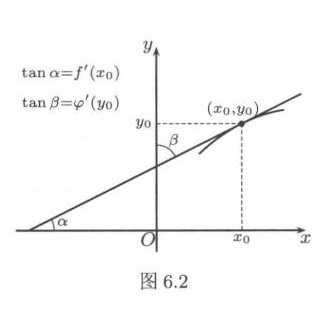
\includegraphics[width=.45\linewidth]{figures/upper/ch06/fig-6-2.png}
\end{center}
\end{xremark}

\begin{xproof}
根据命题 5.5.4（即单调连续函数的反函数定理），$f(x)$ 在点 $x_0$ 的邻近也是严格单调连续函数。从 $x=\varphi(y)$ 在点 $y_0$ 处可导出发，应用公式 (6.3) 得到
\begin{equation}
  \Delta x=x-x_0=[\varphi'(y_0)+\omega(y)](y-y_0)=[\varphi'(y_0)+\omega(y)]\Delta y,
  \tag{6.4}
  \label{eq:6.4}
\end{equation}
其中 $\omega(y)$ 满足条件
\[
  \lim_{y\to y_0}\omega(y)=\omega(y_0)=0.
\]
现在用 $y=f(x)$ 代入等式 (6.4) 中的 $\omega(y)$ 内。由于 $f(x)$ 在 $x_0$ 处连续，而 $\omega(y)$ 在 $y_0=f(x_0)$ 处连续，从复合函数的连续性定理知道 $\omega(f(x))$ 在 $x_0$ 处连续，且有
\[
  \lim_{x\to x_0}\omega(f(x))
  =\omega\!\left(\lim_{x\to x_0}f(x)\right)
  =\omega(f(x_0))=\omega(y_0)=0.
\]
再利用条件 $\varphi'(y_0)\ne0$，存在点 $x_0$ 的某邻域 $O(x_0)$，当 $x\in O(x_0)$ 时，有
\[
  \varphi'(y_0)+\omega(f(x))\ne0.
\]
因此当 $x\in O(x_0)$ 时，可以从 (6.4) 得到
\[
  \frac{\Delta y}{\Delta x}
  =\frac{1}{\varphi'(y_0)+\omega(f(x))}.
\]
令 $x\to x_0$，即 $\Delta x\to0$，就有所要的结果
\[
  \lim_{\Delta x\to0}\frac{\Delta y}{\Delta x}=\frac{1}{\varphi'(y_0)}.
\]
\end{xproof}

\begin{xremark}
对这个结果的常见说法是从
\[
  \frac{\Delta y}{\Delta x}=\frac{1}{\dfrac{\Delta x}{\Delta y}}
\]
取极限，就可以得到
\[
  \frac{\dd y}{\dd x}=\frac{1}{\dfrac{\dd x}{\dd y}}.
\]
这作为一种启发或记忆方法是可以的，但要严格讲清楚的话并不容易。而在上面的证明中只要用公式 (6.3) 进行计算。
\end{xremark}

\begin{xproposition}[6.1.2（复合函数求导的链式法则）]
设 $u=\varphi(x)$ 于 $x_0$ 处可导，$y=f(u)$ 于 $u_0=\varphi(x_0)$ 处可导，则 $y=f(\varphi(x))$ 于 $x_0$ 处可导，而且有
\[
  [f(\varphi(x))]'_{x=x_0}=f'(u_0)\varphi'(x_0).
\]
\end{xproposition}
\begin{xproof}
分别将无穷小增量公式 (6.3) 用于 $u=\varphi(x)$（在 $x_0$）和 $y=f(u)$（在 $u_0$），得到
\begin{align}
  \varphi(x)-\varphi(x_0)&=[\varphi'(x_0)+\omega_1(x)]\Delta x, \tag{6.5}\label{eq:6.5}\\
  f(u)-f(u_0)&=[f'(u_0)+\omega_2(u)]\Delta u, \tag{6.6}\label{eq:6.6}
\end{align}
其中 $\omega_1(x)$ 在 $x_0$ 处连续，且取值为 0，又其中 $\omega_2(u)$ 在 $u_0$ 连续，且取值为 0。

现在考虑复合函数 $y=f(\varphi(x))$。在 (6.6) 中令 $u=\varphi(x)$，利用条件 $u_0=\varphi(x_0)$，从而有 $\Delta u=\varphi(x)-\varphi(x_0)$，然后再将 (6.5) 代入，就得到
\[
  \Delta y=f(\varphi(x))-f(\varphi(x_0))
  =f'(u_0)\varphi'(x_0)\Delta x+\omega(x)\Delta x,
\]
其中
\[
  \omega(x)=f'(u_0)\omega_1(x)+\varphi'(x_0)\omega_2(\varphi(x))+\omega_1(x)\omega_2(\varphi(x)).
\]
根据 $\omega_1(x)$ 和 $\omega_2(u)$ 分别在 $x_0$ 和 $u_0=\varphi(x_0)$ 处连续且取值为 0，又知道 $\varphi(x)$ 在 $x_0$ 处连续，就可以看出函数 $\omega(x)$ 在 $x_0$ 处连续且取值为 0。这样就得到
\[
  \lim_{x\to x_0}\omega(x)=0.
\]
现在只要写出差商
\[
  \frac{\Delta y}{\Delta x}=f'(u_0)\varphi'(x_0)+\omega(x),
\]
再令 $x\to x_0$，就得到所要求证的公式
\[
  [f(\varphi(x))]'_{x=x_0}=f'(u_0)\varphi'(x_0).
\]
\end{xproof}

\begin{xremark}
关于复合函数求导法则证明的一个常见错误是从
\begin{equation}
  \frac{\Delta y}{\Delta x}=\frac{\Delta y}{\Delta u}\cdot\frac{\Delta u}{\Delta x}
  \tag{6.7}
  \label{eq:6.7}
\end{equation}
出发，令 $\Delta x\to0$，得到
\[
  \frac{\dd y}{\dd x}=\frac{\dd y}{\dd u}\cdot\frac{\dd u}{\dd x}.
\]
由于这里涉及对函数极限的基本理解问题，需要作些解释。

在 (6.7) 的左边，按照极限定义有 $\Delta x\ne0$，因此无问题。但在右边的
\[
  \Delta u=u-u_0=\varphi(x)-\varphi(x_0)
\]
完全可能取到 0 值（甚至有可能在 $\Delta x\to0$ 的过程中无限次取到 0 值），因此等式 (6.7) 是不合法的。这里的 $\Delta u$ 是中间变量 $u=\varphi(x)$ 的增量，它是由自变量 $x$ 的增量 $\Delta x$ 决定的，没有理由加上 $\Delta u\ne0$ 的限制。

但在命题 6.1.2 的上述证明中不存在任何概念上的困难，只是有关连续性的普通计算而已。这就是用无穷小增量公式 (6.3) 代替 (6.1) 的优点。
\end{xremark}

\begin{xexample}[6.1.5]
求函数
\[
  f(x)=
  \begin{cases}
    x^2\sin\dfrac1x, & x\ne0,\\[4pt]
    0, & x=0
  \end{cases}
\]
的导函数，并讨论其连续性（参见图 6.3）。
\end{xexample}
\begin{xsolution}
在 $x\ne0$ 处可以用初等函数的求导法则，但在点 $x=0$ 处则必须按导数的定义，先写出差商，再求极限。根据 $f$ 的定义，可得到 $f'(0)=0$（具体计算过程从略）。这里只写出所得的结果：
\[
  f'(x)=
  \begin{cases}
    2x\sin\dfrac1x-\cos\dfrac1x, & x\ne0,\\[4pt]
    0, & x=0.
  \end{cases}
\]

\begin{center}
  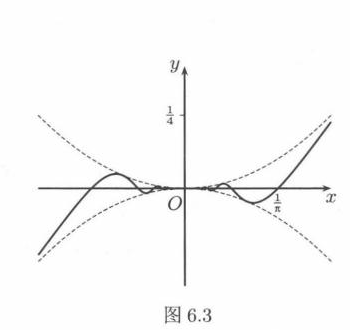
\includegraphics[width=.48\linewidth]{figures/upper/ch06/fig-6-3.png}
\end{center}

由此可见，函数 $f(x)$ 处处可导，但导函数 $f'(x)$ 在点 $x=0$ 处不连续。由于极限 $\lim_{x\to0}f'(x)$ 不存在，因此 $x=0$ 是第二类间断点。
\end{xsolution}

\begin{xremark}
函数在某点的单侧导数和导函数在该点的单侧极限是不同的概念。初学者在这一个问题上容易把两者混淆。对本题来说，既然有 $f'(0)=0$，因此在 $x=0$ 处的两个单侧导数均为 0，即 $f'_-(0)=f'_+(0)=0$。但从 $f'(x)$ 在 $x\ne0$ 时的表达式可以看出，导函数在点 $x=0$ 的两个单侧极限，即 $f'(0^-)$ 和 $f'(0^+)$ 都不存在。（参见下一章的命题 7.1.7，即单侧导数极限定理。）
\end{xremark}

\begin{xexample}[6.1.6]
确定函数
\[
  f(x)=
  \begin{cases}
    ax+b, & x>1,\\
    x^2, & x\le1
  \end{cases}
\]
中的 $a,b$，使得函数 $f(x)$ 在 $x=1$ 处可导。
\end{xexample}
\begin{xsolution}
根据函数在一点存在导数的充分必要条件是两个单侧导数存在且相等，我们将分别计算 $f'_-(1)$ 和 $f'_+(1)$。

左侧导数 $f'_-(1)$ 可以直接计算如下：
\[
  f'_-(1)=\lim_{\Delta x\to0^-}\frac{(1+\Delta x)^2-1}{\Delta x}
  =\lim_{\Delta x\to0^-}\frac{2\Delta x+\Delta^2x}{\Delta x}=2.
\]
右侧导数的计算有所不同。这里一方面涉及两个待定的数 $a,b$，另一方面又必须保证函数在点 $x=1$ 处有连续性。由函数 $f$ 在 $x>1$ 的表达式 $ax+b$ 和 $f(1)=1$ 可见 $a,b$ 必须满足要求 $a+b=1$，否则 $f'_+(1)$ 就不可能存在。令 $b=1-a$，然后可以计算如下：
\[
  f'_+(1)=\lim_{\Delta x\to0^+}\frac{a(1+\Delta x)+(1-a)-1}{\Delta x}
  =\lim_{\Delta x\to0^+}\frac{a\Delta x}{\Delta x}=a.
\]
令 $f'_-(1)=f'_+(1)$，得到 $a=2$，从而 $b=-1$。
\end{xsolution}

\begin{xremark}
由于单侧导数与导函数的单侧极限是不同的概念，因此本题应当按单侧导数的定义计算。注意在求（单侧）导数之前先要看是否（单侧）连续。
\end{xremark}

导数计算中的一个困难是求形式为 $u(x)^{v(x)}$ 的函数的导函数。

\begin{xexample}[6.1.7]
计算 $f(x)=x^{1/x}$ 的导函数。
\end{xexample}
\begin{xsolution}
用对数求导法。先取对数得到
\[
  \ln f(x)=\ln(x^{1/x})=\frac{\ln x}{x},
\]
然后求导，左边用复合函数求导法则得到
\[
  [\ln f(x)]'=\frac{f'(x)}{f(x)},
\]
右边直接计算得到
\[
  \left(\frac1x\cdot\ln x\right)'=-\frac{1}{x^2}\ln x+\frac{1}{x^2}=\frac{1}{x^2}(1-\ln x).
\]
这样就计算出
\[
  f'(x)=f(x)\cdot\frac{1}{x^2}(1-\ln x)=x^{1/x-2}(1-\ln x).
\]
\end{xsolution}

\begin{xremark}
对数求导法在对乘积形式的函数求导数时也有用处。例如设有多项式
\[
  p(x)=(x-x_1)(x-x_2)\cdots(x-x_n),
\]
且其中 $x_i,i=1,2,\ldots,n$ 互不相等，则为了求 $p(x)$ 的导数，可以先取绝对值，再取对数，然后将
\[
  \ln\abs{p(x)}=\ln\abs{x-x_1}+\ln\abs{x-x_2}+\cdots+\ln\abs{x-x_n}
\]
对 $x$ 求导，就很方便地得到
\[
  p'(x)=p(x)\left(\frac1{x-x_1}+\frac1{x-x_2}+\cdots+\frac1{x-x_n}\right).
\]
\end{xremark}

\subsection{练习题}

\begin{xexercise}[1]
证明以下基本事实：
  \begin{enumerate}[label=(\arabic*)]
    \item 可导的偶函数的导函数为奇函数；
    \item 可导的奇函数的导函数为偶函数；
    \item 可导的周期函数的导函数为周期函数。
  \end{enumerate}
\end{xexercise}
\begin{xsolution}
\begin{enumerate}[label=(\arabic*)]
  \item 若 $f$ 为偶函数，则 $f(-x)=f(x)$。对 $x$ 求导，
  \[
    -f'(-x)=f'(x),
  \]
  即 $f'(-x)=-f'(x)$，所以 $f'$ 为奇函数。

  \item 若 $f$ 为奇函数，则 $f(-x)=-f(x)$。求导得
  \[
    -f'(-x)=-f'(x),
  \]
  因而 $f'(-x)=f'(x)$，所以 $f'$ 为偶函数。

  \item 若 $f(x+T)=f(x)$，其中 $T$ 是周期，则两边对 $x$ 求导，得到
  \[
    f'(x+T)=f'(x),
  \]
  故 $f'$ 仍以 $T$ 为周期。
\end{enumerate}
\end{xsolution}


\begin{xexercise}[2]
已知偶函数 $f(x)$ 在点 $x=0$ 处可导，求 $f'(0)$。
\end{xexercise}
\begin{xsolution}
由思考题 9(3)，可导偶函数在原点的导数必为零。因此
\[
  f'(0)=0.
\]
\end{xsolution}


\begin{xexercise}[3]
确定 $a$ 的值，使两条曲线 $y=ax^2$ 与 $y=\ln x$ 相切。
\end{xexercise}
\begin{xsolution}
设两曲线在 $x=x_0>0$ 处相切，则函数值和导数都相等：
\[
  ax_0^2=\ln x_0,
  \qquad
  2ax_0=\frac1{x_0}.
\]
第二式给出
\[
  a=\frac1{2x_0^2}.
\]
代入第一式得
\[
  \frac12=\ln x_0,
\]
故 $x_0=\sqrt{\ee}$，进而
\[
  \boxed{a=\frac1{2\ee}}.
\]
\end{xsolution}


\begin{xexercise}[4]
设函数 $f(x),g(x)$ 在点 $x_0$ 处均可导。证明：$f(x)-g(x)=\littleo(x-x_0)\ (x\to x_0)$ 的充分必要条件是两条曲线 $y=f(x)$ 与 $y=g(x)$ 在 $x=x_0$ 时相切。
\end{xexercise}
\begin{xsolution}
先设
\[
  f(x)-g(x)=\littleo(x-x_0)\qquad(x\to x_0).
\]
由于 $f,g$ 可导，因而连续，令 $x\to x_0$ 可得 $f(x_0)=g(x_0)$。再除以 $x-x_0$ 并取极限：
\[
  \lim_{x\to x_0}\frac{[f(x)-g(x)]-[f(x_0)-g(x_0)]}{x-x_0}=0,
\]
故 $f'(x_0)=g'(x_0)$。于是两曲线在 $(x_0,f(x_0))$ 处有相同切线。

反之，若两曲线在 $x=x_0$ 处相切，则
\[
  f(x_0)=g(x_0),\qquad f'(x_0)=g'(x_0).
\]
对 $h=f-g$ 使用无穷小增量公式，
\[
  h(x)=h(x_0)+h'(x_0)(x-x_0)+\littleo(x-x_0)
  =\littleo(x-x_0),
\]
即得所需条件。
\end{xsolution}


\begin{xexercise}[5]
设函数 $f(x)$ 可导，且 $f(x)$ 无零点。证明：两条曲线 $y=f(x)$ 和 $y=f(x)\sin x$ 在其交点处相切。
\end{xexercise}
\begin{xsolution}
交点满足
\[
  f(x)=f(x)\sin x.
\]
因 $f(x)$ 无零点，必有 $\sin x=1$，即
\[
  x=\frac\pi2+2k\pi,\qquad k\in\ZZ.
\]
设 $g(x)=f(x)\sin x$，则
\[
  g'(x)=f'(x)\sin x+f(x)\cos x.
\]
在交点处 $\sin x=1,\cos x=0$，故
\[
  g'(x)=f'(x).
\]
两曲线在交点处函数值和导数均相同，所以相切。
\end{xsolution}


\begin{xexercise}[6]
设 $p(x)$ 是有 $n$ 个实根的 $n$ 次多项式，记它的相异根为 $x_1,\ldots,x_k$，其中根 $x_i$ 的重数为 $n_i,i=1,2,\ldots,k,n_1+n_2+\cdots+n_k=n$。证明：成立
  \[
    p'(x)=p(x)\left(\sum_{i=1}^k\frac{n_i}{x-x_i}\right).
  \]
\end{xexercise}
\begin{xsolution}
将多项式写成
\[
  p(x)=C\prod_{i=1}^k(x-x_i)^{n_i},\qquad C\ne0.
\]
当 $x\ne x_i$ 时取对数求导：
\[
  \frac{p'(x)}{p(x)}=\sum_{i=1}^k\frac{n_i}{x-x_i}.
\]
于是
\[
  p'(x)=p(x)\sum_{i=1}^k\frac{n_i}{x-x_i}.
\]
右端在约去相应因子后实际上是一个多项式；上式在 $x\ne x_i$ 的稠密集合上成立，因此作为多项式恒等式延拓到所有 $x$。特别地，在根处应理解为约分后的连续延拓值。
\end{xsolution}


\begin{xexercise}[7]
设函数
  \[
    f(x)=
    \begin{cases}
      \dfrac{x}{1+\ee^{1/x}}, & x\ne0,\\[4pt]
      0, & x=0,
    \end{cases}
  \]
  研究 $f(x)$ 的可导性。
\end{xexercise}
\begin{xsolution}
当 $x\ne0$ 时，$f$ 是初等函数，故可导。只需考察 $x=0$。

先看连续性。若 $x\to0^+$，则
\[
  0\le \frac{x}{1+\ee^{1/x}}\le x\ee^{-1/x}\to0.
\]
若 $x\to0^-$，则 $\ee^{1/x}\to0$，从而
\[
  \frac{x}{1+\ee^{1/x}}\sim x\to0.
\]
故 $f$ 在 $0$ 连续。

导数差商为
\[
  \frac{f(x)-f(0)}x=\frac1{1+\ee^{1/x}}.
\]
于是
\[
  \lim_{x\to0^+}\frac{f(x)}x=0,
  \qquad
  \lim_{x\to0^-}\frac{f(x)}x=1.
\]
左右导数不相等，所以 $f'(0)$ 不存在。故 $f$ 恰在 $\RR\setminus\{0\}$ 上可导。
\end{xsolution}


\begin{xexercise}[8]
设 $n$ 为正整数，在什么条件下，函数
  \[
    f(x)=
    \begin{cases}
      x^n\sin\dfrac1x, & x\ne0,\\[4pt]
      0, & x=0
    \end{cases}
  \]
  (1) 在 $x=0$ 处连续；(2) 在 $x=0$ 处可导；(3) 在 $x=0$ 处导函数连续。
\end{xexercise}
\begin{xsolution}
$n$ 为正整数。

(1) 因
\[
  \abs{x^n\sin\frac1x}\le\abs{x}^n\to0,
\]
所以对每个 $n\ge1$，$f$ 都在 $0$ 连续。

(2) 差商为
\[
  \frac{f(x)-f(0)}x=x^{n-1}\sin\frac1x.
\]
当 $n\ge2$ 时其极限为 $0$；当 $n=1$ 时极限不存在。因此在 $0$ 可导当且仅当
\[
  \boxed{n\ge2},\qquad f'(0)=0.
\]

(3) 对 $x\ne0$，
\[
  f'(x)=n x^{n-1}\sin\frac1x-x^{n-2}\cos\frac1x.
\]
当 $n\ge3$ 时两项都趋于 $0=f'(0)$，故 $f'$ 在 $0$ 连续；$n=2$ 时第二项为 $-\cos(1/x)$，极限不存在。因此导函数在 $0$ 连续当且仅当
\[
  \boxed{n\ge3}.
\]
\end{xsolution}


\begin{xexercise}[9]
设函数 $f(x)$ 满足函数方程 $f(x+y)=f(x)\cdot f(y)$，且已知 $f'(0)=1$。证明：$f(x)$ 处处可导，且成立 $f'(x)=f(x)$。（可与 5.1.4 小节的题 10 作比较。）
\end{xexercise}
\begin{xsolution}
由函数方程取 $x=y=0$，得 $f(0)=f(0)^2$。又因 $f'(0)=1$，$f$ 不可能恒为零，所以 $f(0)=1$。

对任意固定 $x$，有
\[
  \frac{f(x+h)-f(x)}h
  =\frac{f(x)f(h)-f(x)}h
  =f(x)\frac{f(h)-1}h.
\]
令 $h\to0$，由 $f'(0)=1$ 得
\[
  f'(x)=f(x)f'(0)=f(x).
\]
因此 $f$ 处处可导，且 $f'(x)=f(x)$。
\end{xsolution}


\begin{xexercise}[10]
给定函数
  \[
    f(x)=\begin{cases}0,&x\text{ 为无理数},\\x,&x\text{ 为有理数},\end{cases}
    \qquad
    g(x)=\begin{cases}0,&x\text{ 为无理数},\\x^2,&x\text{ 为有理数},\end{cases}
  \]
  讨论它们的连续性与可导性。
\end{xexercise}
\begin{xsolution}
对
\[
  f(x)=\begin{cases}0,&x\notin\QQ,\\x,&x\in\QQ,
  \end{cases}
\]
若 $x_0\ne0$，沿有理数趋于 $x_0$ 时函数值趋于 $x_0$，沿无理数趋于 $x_0$ 时函数值趋于 $0$，故不连续。只有在 $x_0=0$ 时两类序列都使 $f(x)\to0$，所以 $f$ 仅在 $0$ 连续。其在 $0$ 的差商为
\[
  \frac{f(h)}h=\begin{cases}0,&h\notin\QQ,\\1,&h\in\QQ,
  \end{cases}
\]
极限不存在，故 $f$ 处处不可导。

对
\[
  g(x)=\begin{cases}0,&x\notin\QQ,\\x^2,&x\in\QQ,
  \end{cases}
\]
同理，$g$ 仅在 $0$ 连续。且
\[
  \frac{g(h)-g(0)}h=
  \begin{cases}
    0,&h\notin\QQ,\\
    h,&h\in\QQ,
  \end{cases}
  \longrightarrow0.
\]
故 $g'(0)=0$；在其他点因不连续而不可导。因此 $g$ 恰在 $0$ 可导。
\end{xsolution}


\begin{xexercise}[11]
设
  \[
    f(x)=\begin{cases}x,&x\text{ 为有理数},\\x^2+x,&x\text{ 为无理数}.
    \end{cases}
  \]
  (1) 证明 $x\ne0$ 时，$f$ 不连续；(2) 计算 $f'(0)$。
\end{xexercise}
\begin{xsolution}
(1) 设 $x_0\ne0$。沿有理数 $x\to x_0$，$f(x)\to x_0$；沿无理数 $x\to x_0$，$f(x)\to x_0^2+x_0$。两极限相等要求 $x_0^2=0$，与 $x_0\ne0$ 矛盾。因此 $x_0\ne0$ 时 $f$ 不连续。

(2) $f(0)=0$。当 $h\ne0$ 时
\[
  \frac{f(h)-f(0)}h=
  \begin{cases}
    1,&h\in\QQ,\\
    1+h,&h\notin\QQ.
  \end{cases}
\]
两种情形在 $h\to0$ 时都趋于 $1$，故
\[
  \boxed{f'(0)=1}.
\]
\end{xsolution}


\begin{xexercise}[12]
设在原点某邻域 $O(0)$ 上有 $\abs{f(x)}\le\abs{g(x)}$，且 $g(0)=g'(0)=0$。求 $f'(0)$。
\end{xexercise}
\begin{xsolution}
由 $g(0)=0$ 和 $\abs{f(0)}\le\abs{g(0)}$ 得 $f(0)=0$。又因 $g'(0)=0$，
\[
  \lim_{x\to0}\frac{g(x)}x=0.
\]
于是对 $x\ne0$，
\[
  \abs{\frac{f(x)-f(0)}x}
  =\abs{\frac{f(x)}x}
  \le\abs{\frac{g(x)}x}\to0.
\]
由夹逼定理，
\[
  \boxed{f'(0)=0}.
\]
\end{xsolution}


% END OF SECTION 6.1 TRANSCRIPTION

\section{高阶导数及其他求导法则}

本节的内容为高阶导数的计算方法、隐函数求导法则和用参数方程给出的函数的求导法则。

\subsection{高阶导数计算}

高阶导数的计算，特别是 $n$ 阶导数的一般表达式的计算往往会有困难，这里 Leibniz（莱布尼茨）公式是主要工具：
\[
  (uv)^{(n)}
  =\binom n0u^{(0)}v^{(n)}+\binom n1u'v^{(n-1)}+\binom n2u''v^{(n-2)}+\cdots+\binom nn u^{(n)}v^{(0)}
  =\sum_{k=0}^n\binom nk u^{(k)}v^{(n-k)}.
\]
由于这个公式在各种教科书中都有证明，这里不再重复。

在 Leibniz 公式的右边有 $n+1$ 项，如果在 $uv$ 中有一个函数是低次多项式，则实际出现的项数就很少，这对于计算很有利。

\begin{xexample}[6.2.1]
计算 $(x^2\sin x)^{(80)}$。
\end{xexample}
\begin{xsolution}
用 Leibniz 公式和 $(\sin x)^{(4)}=\sin x,(\cos x)^{(4)}=\cos x$，就有
\[
\begin{aligned}
  (x^2\sin x)^{(80)}
  &=x^2(\sin x)^{(80)}+\binom{80}{1}(x^2)'(\sin x)^{(79)}\\
  &\quad+\binom{80}{2}(x^2)''(\sin x)^{(78)}\\
  &=(x^2-6320)\sin x-160x\cos x.
\end{aligned}
\]
\end{xsolution}

\begin{xexample}[6.2.2]
设 $f(x)=\dfrac{2x}{1-x^2}$，求 $f^{(n)}(x)$。
\end{xexample}
\begin{xsolution}
分解为简单分式后再求导。先将 $f$ 改写为
\[
  f(x)=\frac1{1-x}-\frac1{1+x},
\]
这样就有
\[
  f^{(n)}(x)=\left(\frac1{1-x}\right)^{(n)}-\left(\frac1{1+x}\right)^{(n)}.
\]
然后可以试求几次找出规律，并用数学归纳法证明（细节从略）：
\[
  \left(\frac{2x}{1-x^2}\right)^{(n)}
  =n!\left[\frac1{(1-x)^{n+1}}-\frac{(-1)^n}{(1+x)^{n+1}}\right].
\]
\end{xsolution}

\begin{xexample}[6.2.3]
对 $y=\arcsin x$ 计算 $y^{(n)}(0)$。
\end{xexample}
\begin{xsolution}
直接计算很难总结出规律。关键是寻找递推关系。首先有
\[
  y'=\frac1{\sqrt{1-x^2}},
\]
将它改写为
\[
  y'\sqrt{1-x^2}=1
\]
后再求导，得到
\[
  y''\sqrt{1-x^2}-y'\cdot\frac{x}{\sqrt{1-x^2}}=0.
\]
又将它整理为
\[
  (1-x^2)y''-xy'=0,
\]
然后用 Leibniz 公式得到
\[
  y^{(n+2)}(1-x^2)+ny^{(n+1)}(-2x)+\frac{n(n-1)}2y^{(n)}(-2)
  -(xy^{(n+1)}+ny^{(n)})=0.
\]
整理后得到
\[
  (1-x^2)y^{(n+2)}-(2n+1)xy^{(n+1)}-n^2y^{(n)}=0.
\]
现在用 $x=0$ 代入，就得到递推公式
\[
  y^{(n+2)}(0)-n^2y^{(n)}(0)=0.
\]
从 $y(0)=0$ 即可知道 $y(x)$ 在 $x=0$ 的所有偶数阶导数都等于零：$y^{(2k)}(0)=0,k\in\NN_+$。再从 $y'(0)=1$ 出发用递推公式，计算出 $y'''(0)=1,y^{(5)}(0)=3^2,y^{(7)}(0)=5^2\cdot3^2,\ldots$，即可总结出
\[
  y^{(2k+1)}(0)=[(2k-1)!!]^2,\qquad k\in\NN_+.
\]
\end{xsolution}

\begin{xremark}
在第七章学了 Taylor 公式后可以提出一种计算高阶导数的间接方法。见那里的例题 7.2.1 解 1 之后的注解中对本题的回顾。
\end{xremark}

\begin{xexample}[6.2.4]
设
\[
  f(x)=
  \begin{cases}
    \ee^{-1/x^2}, & x\ne0,\\
    0, & x=0,
  \end{cases}
\]
证明 $f^{(n)}(0)=0,n\in\NN_+$（见图 6.4）。
\end{xexample}

\begin{center}
  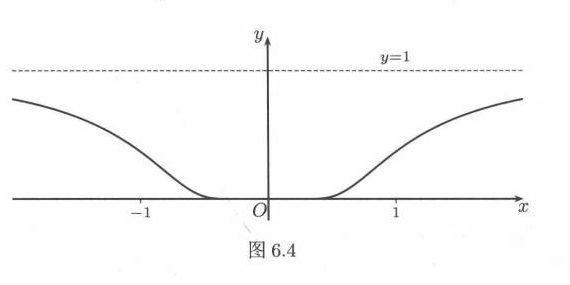
\includegraphics[width=.68\linewidth]{figures/upper/ch06/fig-6-4.png}
\end{center}

\begin{xproof}
这里的基础是对于任何 $\alpha$ 成立
\[
  \lim_{u\to+\infty}\frac{u^\alpha}{\ee^u}=0.
\]
先计算 $f'(0)$。按定义计算并作代换 $y=1/x$，就有
\[
  f'(0)=\lim_{x\to0}\frac1x\cdot\ee^{-1/x^2}=\lim_{y\to\infty}y\ee^{-y^2}=0.
\]
然后求出 $x\ne0$ 时的导函数表达式
\[
  f'(x)=\frac{2}{x^3}\cdot\ee^{-1/x^2},
\]
再按定义计算出
\[
  f''(0)=\lim_{x\to0}\frac{f'(x)-f'(0)}x
  =\lim_{x\to0}\frac{2}{x^4}\cdot\ee^{-1/x^2}=0.
\]
然后求出 $x\ne0$ 时的二阶导函数表达式
\[
  f''(x)=\left(\frac4{x^6}-\frac6{x^4}\right)\cdot\ee^{-1/x^2}.
\]
可以提出猜测，即函数 $f$ 的 $n$ 阶导数在 $x\ne0$ 时具有以下形式：
\[
  f^{(n)}(x)=P_n\!\left(\frac1x\right)\cdot\ee^{-1/x^2},
\]
其中的 $P_n(1/x)$ 的意义是在变量 $y$ 的多项式 $P_n(y)$ 中用 $y=1/x$ 代入。由于我们只要求计算 $f^{(n)}(0)$，而从前面的两次计算可以知道，我们不必去关心多项式 $P_n(y)$ 的具体次数、系数和递推关系。

用数学归纳法来证明这个猜测。已看到 $n=1,2$ 时猜测成立。设 $f^{(k)}(x)$ 已具有所说的形式，讨论 $f^{(k+1)}(x)$。通过对 $f^{(k)}(x)$ 求导，就有
\begin{align*}
  f^{(k+1)}(x)
  &=\left(P_k\!\left(\frac1x\right)\ee^{-1/x^2}\right)'\\
  &=P_k'\!\left(\frac1x\right)\left(-\frac1{x^2}\right)\ee^{-1/x^2}
    +P_k\!\left(\frac1x\right)\left(\frac2{x^3}\right)\ee^{-1/x^2}\\
  &=\left[P_k'(y)(-y^2)+P_k(y)(2y^3)\right]_{y=1/x}\ee^{-1/x^2},
\end{align*}
将第一个因子记为 $P_{k+1}(1/x)$ 即可。

最后，用数学归纳法来证明对于任意的正整数 $n$，有 $f^{(n)}(0)=0$ 成立。在 $n=1,2$ 时已经成立。设在 $n=k$ 时已有 $f^{(k)}(0)=0$，则对于 $n=k+1$，可以利用 $n=k$ 和 $x\ne0$ 时 $f^{(k)}(x)$ 的上述特殊形式作以下计算：
\[
  f^{(k+1)}(0)
  =\lim_{x\to0}\frac{f^{(k)}(x)-f^{(k)}(0)}x
  =\lim_{x\to0}\frac{f^{(k)}(x)}x
  =\lim_{x\to0}\frac1xP_k\!\left(\frac1x\right)\ee^{-1/x^2}=0.
\]
\end{xproof}

\begin{xremark}
这是在数学分析中的重要例子。(1) 它说明一个非常值函数也可以在某些点上的任何阶导数等于 0；(2) 幂函数 $x^n\ (n\ge2)$ 在 $x=0$ 处直到 $n-1$ 阶的导数均为 0，当 $x\to0$ 时为 $n$ 阶无穷小量。因此 $x^n$ 的图像在原点附近随着 $n$ 增加越来越平坦。但是与本例的函数相比，就大为不如。因为这里对所有 $n$ 都成立
\[
  \ee^{-1/x^2}=\littleo(x^n)\quad(x\to0).
\]
从图 6.4 可见这个函数在 $x=0$ 附近的图像极其平坦。(3) 在 Taylor 公式（§7.2）和 Taylor 级数（见下册命题 14.4.2）的理论中，本例的函数有重要的应用。

下一个例题说明：上述例子不只是理论上的“精品”，而且有实际上的价值，其中的辅助函数在许多研究中有用。
\end{xremark}

\begin{xexample}[6.2.5]
将 $(-\infty,0]$ 上的常值函数 $u(x)\equiv0$ 和 $[1,+\infty)$ 上的常值函数 $v(x)\equiv1$ 延拓为在 $(-\infty,+\infty)$ 上的无限次可微函数，且使其值域为 $[0,1]$。
\end{xexample}
\begin{xsolution}
先定义
\[
  g(x)=
  \begin{cases}
    0, & x\le0,\\
    \ee^{-1/x^2}, & x>0,
  \end{cases}
\]
然后令
\[
  f(x)=\frac{g(x)}{g(x)+g(1-x)},
\]
则 $f(x)$ 就满足要求。（请读者验证。）
\end{xsolution}

\subsection{隐函数求导法}

从上一章的命题 5.5.4 和其后的两个例题中我们已经看到，函数的给定方法已经突破了过去的显式方法，而可以采用隐式方法。具体地说，再举那里的 Kepler 方程为例，即可以用一个方程
\[
  y=x-q\sin x\qquad(0<q<1)
\]
来定义一个函数 $x=x(y)$。用第二、三章中的迭代生成数列的方法可以计算这个函数（的近似值）。在上一章我们能够确定这个函数是连续单调增加函数，而在本章则从反函数求导法则（即命题 6.1.1）还知道它可导，且可以将导数 $x'(y)$ 计算出来（看下面的例题 6.2.6）。

本小节的隐函数求导法则与多元函数的偏导数计算有关，它的一般形式将在多元微积分的隐函数章节中学习。在这里只介绍这个法则的基本思想，并计算一些较为简单的问题。

这里的要点是：如果一个函数 $y=y(x)$ 满足方程
\[
  F(x,y)=0,
\]
则将它代入后就得到恒等式 $F(x,y(x))\equiv0$。然后对 $x$ 求导，就有可能将导数 $y'(x)$ 计算出来。

可以认为隐函数求导法则是反函数求导法则的一个发展。实际上根据上述思想就可以导出反函数的求导法则如下。

若 $y=y(x)$ 和 $x=x(y)$ 互为反函数，则可将 $y=y(x)$ 代入后者，得到
\[
  x=x(y(x)).
\]
对 $x$ 求导，就有
\[
  1=x'(y(x))y'(x),
\]
这样就可以得到反函数求导公式
\[
  y'(x)=\frac1{x'(y)},
\]
其中 $y=y(x)$ 由 $x=x(y)$ 决定。（这不能代替命题 6.1.1。为什么？）

\begin{xexample}[6.2.6]
设函数 $x=x(y)$ 满足 Kepler 方程 $y=x-q\sin x\ (0<q<1)$，求 $x'(y)$。
\end{xexample}
\begin{xsolution}
解 1\quad 已知 $y=x-q\sin x\ (0<q<1)$ 是以 $(-\infty,+\infty)$ 为定义域和值域的连续单调增加函数。由于导数 $y'=1-q\cos x\ne0$，就可以应用命题 6.1.1，知道反函数 $x(y)$ 可导，且得到导数
\[
  x'(y)=\frac1{y'(x)}=\frac1{1-q\cos x(y)}.
\]

解 2\quad 将函数 $x=x(y)$ 代入方程 $y-x+q\sin x=0$ 中，得到以 $y$ 为自变量的恒等式
\[
  y-x(y)+q\sin x(y)=0.
\]
对 $y$ 求导，得到
\[
  1-x'(y)+q\cos x(y)\cdot x'(y)=0.
\]
这样就可以得到
\[
  x'(y)=\frac1{1-q\cos x(y)}.
\]
\end{xsolution}

\begin{xremark}
对这两个方法进行比较。

第一种解法是严格的，反函数的存在是由命题 5.5.4 保证的，而反函数的可导与计算方法是以命题 6.1.1 为根据的。它的缺点是不能解决一般的隐函数的存在和求导问题。

第二种解法的优点是可以用于一般的隐函数求导计算。但在这一章中对隐函数的存在性和可导性都还不可能建立严格的理论基础，这些问题要到多元微积分中才能解决，在那里会证明这里的计算方法是正确的（见下册的第二十章）。此外，在一般计算中上述恒等式只写成为普通的等式。

现在举一个简单的例子，从中可以看出隐函数求导方法的一个优点。
\end{xremark}

\begin{xexample}[6.2.7]
设函数 $y=y(x)$ 满足单位圆方程 $x^2+y^2=1$，用显式和隐式两种方法求 $y'(x)$，并作比较。
\end{xexample}
\begin{xsolution}
从所给方程可以得到两个显函数：记为
\begin{equation}
  y_1=\sqrt{1-x^2}\quad\text{和}\quad y_2=-\sqrt{1-x^2},\qquad -1\le x\le1.
  \tag{6.8}
  \label{eq:6.8}
\end{equation}
它们在 $-1<x<1$ 上处处可导。容易计算出
\begin{equation}
  y_1'=-\frac{x}{\sqrt{1-x^2}}\quad\text{和}\quad
  y_2'=\frac{x}{\sqrt{1-x^2}}.
  \tag{6.9}
  \label{eq:6.9}
\end{equation}
另一方面，用隐函数求导法则，将 $y=y(x)$ 代入方程，有恒等式
\[
  x^2+y^2(x)\equiv1.
\]
对 $x$ 求导，得到 $2x+2y(x)y'(x)=0$，就有
\begin{equation}
  y'(x)=-\frac{x}{y(x)}.
  \tag{6.10}
  \label{eq:6.10}
\end{equation}
现比较这两个不同的方法。从前面的计算可见，方程 $x^2+y^2=1$ 确定的函数不止一个。实际上，根据函数的定义，两个函数只要定义域不同，即使解析表达式相同，也应当看成是不同的函数。因此从这个观点看的话，方程 $x^2+y^2=1$ 所确定的函数就不是只有两个，而是多得不计其数了。（这正是将来要学习的隐函数理论中的观点。）那么就产生了一个问题，即第二个方法所得的公式 (6.10) 中的 $y'(x)$ 是指哪一个函数 $y(x)$ 的导数？

这个问题的回答是：用隐函数求导法则所得到的导数公式对（由方程确定的）每一个函数同时有效。由于本题十分简单，只要在公式 (6.10) 中用公式 (6.8) 中的 $y_1(x)$ 和 $y_2(x)$ 分别代入，就可以分别得到用第一个方法计算出来的 $y_1'$ 和 $y_2'$，即公式 (6.9)。至于由单位圆方程确定的其他函数，它们的定义域都是 $[-1,1]$ 的子集，因此只要可导，公式 (6.10) 同样有效。
\end{xsolution}

\begin{xexample}[6.2.8]
设 $y=y(x)$ 可导，且满足方程 $x^2+xy+y^2=1$，求 $y',y'',y'''$。
\end{xexample}
\begin{xsolution}
将 $x^2+xy+y^2=1$ 看成关于 $x$ 的恒等式，其中 $y=y(x)$，对 $x$ 求导得到
\begin{equation}
  2x+y+xy'+2yy'=0,
  \tag{6.11}
  \label{eq:6.11}
\end{equation}
就有
\[
  y'=-\frac{2x+y}{x+2y}.
\]
根据这个表达式可以直接看出，在函数 $y(x)$ 可导的假定下，只要分母 $x+2y\ne0$，二阶导数 $y''$ 一定存在。

将 (6.11)（它实际上也是关于 $x$ 的恒等式）对 $x$ 求导，得到
\[
  2+2y'+xy''+2y'^2+2yy''=0.
\]
由此可以计算出（请读者补充计算过程）
\[
  y''=-\frac6{(x+2y)^3}.
\]
从这个公式又一次推知，只要 $x+2y\ne0$，函数 $y(x)$ 就会有三阶导数。对 $y''$ 的公式再求导，就得到
\[
  y'''=-\frac{54x}{(x+2y)^5}.
\]
\end{xsolution}

\begin{xremark}
从平面解析几何的二次曲线理论可知，如图 6.5 所示，本题方程的几何图像是一个以原点为中心的椭圆，但其主轴与坐标轴不重合。这个椭圆与直线 $x+2y=0$ 的交点处的切线平行于 $y$ 轴，斜率为无穷大。当然可以从方程出发得到 $y(x)$ 的显式，但这时的显式表达式较复杂，计算并不方便。而且我们也不知道题意中的 $y(x)$ 是哪一个，因而隐函数求导法则即使在能求出函数的显式公式时也有它的优点。

\begin{center}
  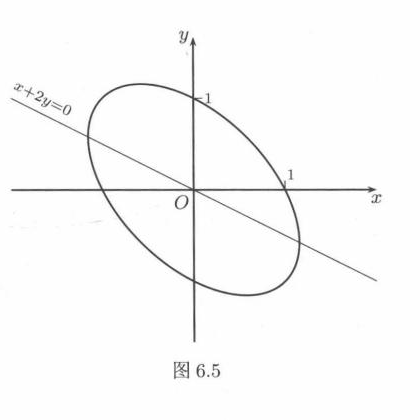
\includegraphics[width=.48\linewidth]{figures/upper/ch06/fig-6-5.png}
\end{center}
\end{xremark}

\subsection{参数方程求导法}

用参数方程给出平面或空间曲线的做法由来已久。从解析几何的发展开始，许多有实际意义的曲线都是这样给定的，如果一定要用 $y=y(x)$ 或 $x=x(y)$ 来表示它们反而会很不方便。这即使对于常见的圆也是如此。在中学里已经学过极坐标和用 $\rho=\rho(\theta)$ 来表示的曲线。若写出
\[
  x=\rho(\theta)\cos\theta,\qquad y=\rho(\theta)\sin\theta,
\]
就得到了以 $\theta$ 为参数的参数方程。

对于一般的参数方程
\[
  x=\varphi(t),\qquad y=\psi(t),\qquad a\le t\le b,
\]
在一定的条件下可以确定函数关系 $y=y(x)$（或 $x=x(y)$）。这时对函数 $y=y(x)$ 的研究完全可以从参数方程出发来进行，而不一定需要 $y=y(x)$ 的显式表达式，因为这样的显式表达式一般地说不一定存在，而即使存在也不一定有用。这里的情况与上一个小节完全类似。

\begin{xproposition}[6.2.1]
设 $x=\varphi(t),y=\psi(t)$ 在区间 $(a,b)$ 上可导，且 $\varphi'(t)\ne0,\forall t\in(a,b)$，则有以下结论成立：
\begin{enumerate}[label=(\arabic*)]
  \item $x=\varphi(t)$ 是区间 $(a,b)$ 上的严格单调连续函数，因而存在反函数 $t=t(x)$；
  \item 在 $x=\varphi(t)$ 和 $y=\psi(t)$ 之间存在函数关系 $y=\psi(t(x))$，简记为 $y=y(x)$；
  \item 函数 $y=y(x)$ 可导，且有公式
  \[
    y'(x)=\left.\frac{\psi'(t)}{\varphi'(t)}\right|_{t=t(x)}.
  \]
\end{enumerate}
\end{xproposition}
\begin{xproof}
关于 (1) 的证明见注 2 的说明，在这里暂且先承认它。(2) 是 (1) 的推论。下面只对 (3) 给出证明。

由 $\varphi'(t)\ne0$ 和 (1)，可以用反函数求导法则（即命题 6.1.1），知道 $t=t(x)$ 可导，且有
\[
  t'(x)=\left.\frac1{\varphi'(t)}\right|_{t=t(x)}.
\]
对 $y=\psi(t(x))$ 用复合函数求导公式，就有
\[
  y'(x)=\psi'(t(x))\cdot t'(x)
  =\left.\frac{\psi'(t)}{\varphi'(t)}\right|_{t=t(x)}.
\]
\end{xproof}

\begin{xremark}
注 1\quad 以上法则可以写为
\[
  y'_x=y'_t t'_x=\frac{y'_t}{x'_t},
\]
因此是复合函数求导公式与反函数求导公式的结合。

注 2\quad 关于 (1) 的证明在此作个说明。由于在区间 $(a,b)$ 上处处有 $\varphi'(t)\ne0$，应用下一章命题 7.1.6 的导函数介值定理（Darboux（达布）定理），可见导函数 $\varphi'(t)$ 在区间 $(a,b)$ 上保号。然后再用第八章 §8.2 中关于单调性的讨论即可。
\end{xremark}

\begin{xexample}[6.2.9]
将例题 6.2.8 中的椭圆用参数方程表示为
\[
  x=\frac2{\sqrt3}\cos t,\qquad y=\sin t-\frac1{\sqrt3}\cos t,
\]
计算 $y$ 对 $x$ 的前三阶导数：$y'_x,y''_x,y'''_x$。
\end{xexample}
\begin{xsolution}
由上面的注解，可以计算如下：
\begin{align*}
  y'_x
  &=\left(\sin t-\frac1{\sqrt3}\cos t\right)'_x
   =\left(\sin t-\frac1{\sqrt3}\cos t\right)'_t\,t'_x\\
  &=\left(\cos t+\frac1{\sqrt3}\sin t\right)\frac1{x'_t}
   =-\frac{\sqrt3}{2}\cot t-\frac12,\\
  y''_x
  &=(y'_x)'_x=(y'_x)'_t\,t'_x
   =\frac{\sqrt3}{2}\csc^2t\cdot\frac1{x'_t}
   =-\frac34\csc^3t,\\
  y'''_x
  &=(y''_x)'_x=(y''_x)'_t\,t'_x
   =-\frac{9\sqrt3}{8}\cdot\frac{\cos t}{\sin^5t}.
\end{align*}
当然在三个答案中的 $t$ 都应当理解为反函数 $t=t(x)=\arccos\frac{\sqrt3}{2}x$。同时只有当分母中的 $\sin t\ne0$ 时公式有效，从 $x'_t=-\frac2{\sqrt3}\sin t$ 可知这就是在推导法则时的条件。实际上有 $x+2y=2\sin t$，因此与例题 6.2.8 一致。
\end{xsolution}

\subsection{练习题}

\begin{xexercise}[1]
对 $y=\arctan x$ 计算 $y^{(n)}(0)$。
\end{xexercise}
\begin{xsolution}
令 $y=\arctan x$，则 $(1+x^2)y'=1$。记 $a_m=y^{(m)}(0)$。对上式求 $n$ 阶导数并令 $x=0$，当 $n\ge1$ 时得到
\[
  a_{n+1}+n(n-1)a_{n-1}=0.
\]
又 $a_1=1,a_2=0$。递推可得
\[
  \boxed{
  y^{(n)}(0)=
  \begin{cases}
    0,&n\text{ 为偶数},\\
    (-1)^{(n-1)/2}(n-1)!,&n\text{ 为奇数}.
  \end{cases}}
\]
\end{xsolution}


\begin{xexercise}[2]
对 $y=(\arctan x)^2$ 计算 $y^{(n)}(0)$。
\end{xexercise}
\begin{xsolution}
令 $u=(\arctan x)^2$。由于 $u$ 为偶函数，所有奇数阶导数在 $0$ 处均为零。由
\[
  (1+x^2)u'=2\arctan x
\]
出发。记 $b_m=u^{(m)}(0)$，并使用上一题的
\[
  a_{2m-1}=(\arctan x)^{(2m-1)}\big|_{x=0}
  =(-1)^{m-1}(2m-2)!.
\]
对 $(1+x^2)u'=2\arctan x$ 求 $2m-1$ 阶导数并令 $x=0$，得到
\[
  b_{2m}+(2m-1)(2m-2)b_{2m-2}
  =2(-1)^{m-1}(2m-2)!.
\]
从 $b_2=2$ 开始归纳。若
\[
  b_{2m-2}=2(-1)^{m-2}(2m-3)!
  \sum_{j=0}^{m-2}\frac1{2j+1},
\]
则代入递推式即得
\[
  b_{2m}=2(-1)^{m-1}(2m-1)!
  \left(\sum_{j=0}^{m-2}\frac1{2j+1}+\frac1{2m-1}\right).
\]
因此
\[
  \boxed{
  u^{(n)}(0)=
  \begin{cases}
    0,&n\text{ 为奇数},\\[3pt]
    \displaystyle 2(-1)^{m-1}(2m-1)!\sum_{j=0}^{m-1}\frac1{2j+1},&n=2m.
  \end{cases}}
\]
\end{xsolution}


\begin{xexercise}[3]
对 $y=(\arcsin x)^2$ 计算 $y^{(n)}(0)$。
\end{xexercise}
\begin{xsolution}
令 $u=(\arcsin x)^2$。直接计算得到
\[
  (1-x^2)u''-xu'=2.
\]
$u$ 为偶函数，所以奇数阶导数在 $0$ 处全为零。记 $b_m=u^{(m)}(0)$。对上式求 $n$ 阶导数并令 $x=0$，当 $n\ge1$ 时有
\[
  b_{n+2}=n^2b_n.
\]
又 $b_2=2$，故
\[
  b_{2m}=2\bigl(2\cdot4\cdots(2m-2)\bigr)^2
  =2^{2m-1}[(m-1)!]^2.
\]
即
\[
  \boxed{
  u^{(n)}(0)=
  \begin{cases}
    0,&n\text{ 为奇数},\\
    2^{2m-1}[(m-1)!]^2,&n=2m.
  \end{cases}}
\]
\end{xsolution}


\begin{xexercise}[4]
设 $y=x^{n-1}\ee^{1/x}$，证明：$y^{(n)}=\dfrac{(-1)^n}{x^{n+1}}\ee^{1/x}$。
\end{xexercise}
\begin{xsolution}
记 $F_n(x)=x^{n-1}\ee^{1/x}$。对 $n$ 归纳证明
\[
  F_n^{(n)}(x)=(-1)^nx^{-n-1}\ee^{1/x}.
\]
$n=1$ 时直接成立。若对 $n$ 成立，则 $F_{n+1}=xF_n$，由 Leibniz 公式
\[
  F_{n+1}^{(n+1)}=xF_n^{(n+1)}+(n+1)F_n^{(n)}.
\]
而
\[
  F_n^{(n+1)}=(-1)^n\ee^{1/x}
  \left(-(n+1)x^{-n-2}-x^{-n-3}\right).
\]
代入后第一类项抵消，得到
\[
  F_{n+1}^{(n+1)}=(-1)^{n+1}x^{-n-2}\ee^{1/x},
\]
归纳完成。
\end{xsolution}


\begin{xexercise}[5]
求下列函数的 $n$ 阶导函数：
  \begin{enumerate}[label=(\arabic*)]
    \item $y=\sin^3x$；
    \item $y=\ee^x\sin x$；
    \item $y=x^{n-1}\ln x$；
    \item $y=x^3\ee^x$；
    \item $y=\dfrac{x^n}{1-x}$；
    \item $y=\dfrac{x^n}{(x+1)^2}$；
    \item $y=\sin ax\sin bx$。
  \end{enumerate}
\end{xexercise}
\begin{xsolution}
\begin{enumerate}[label=(\arabic*)]
  \item 由 $\sin^3x=(3\sin x-\sin3x)/4$，
  \[
    \boxed{y^{(n)}=\frac14\left[3\sin\left(x+\frac{n\pi}{2}\right)-3^n\sin\left(3x+\frac{n\pi}{2}\right)\right]}.
  \]
  \item
  \[
    \boxed{y^{(n)}=2^{n/2}\ee^x\sin\left(x+\frac{n\pi}{4}\right)}.
  \]
  \item
  \[
    \boxed{y^{(n)}=\frac{(n-1)!}{x}},\qquad x>0.
  \]
  \item
  \[
    \boxed{y^{(n)}=\ee^x\left[x^3+3nx^2+3n(n-1)x+n(n-1)(n-2)\right]}.
  \]
  \item 由 $x^n/(1-x)=1/(1-x)-(1+x+\cdots+x^{n-1})$，
  \[
    \boxed{y^{(n)}=\frac{n!}{(1-x)^{n+1}}},\qquad x\ne1.
  \]
  \item 利用
  \[
    \frac{x^n}{(1+x)^2}=n\frac{x^{n-1}}{1+x}-\left(\frac{x^n}{1+x}\right)',
  \]
  以及对 $x^{n-1}/(1+x)$、$x^n/(1+x)$ 作多项式除法后只保留其有理余项，可得
  \[
    \boxed{y^{(n)}=\frac{n!(1-nx)}{(1+x)^{n+2}}},\qquad x\ne-1.
  \]
  \item 由积化和差公式，
  \[
    \boxed{y^{(n)}=\frac12\left[(a-b)^n\cos\left((a-b)x+\frac{n\pi}{2}\right)-(a+b)^n\cos\left((a+b)x+\frac{n\pi}{2}\right)\right]}.
  \]
\end{enumerate}
\end{xsolution}


\begin{xexercise}[6]
证明：$y=C_1\ee^{\lambda_1x}+C_2\ee^{\lambda_2x}$ 满足微分方程 $y''-(\lambda_1+\lambda_2)y'+\lambda_1\lambda_2y=0$。
\end{xexercise}
\begin{xsolution}
逐项求导：
\[
  y'=C_1\lambda_1\ee^{\lambda_1x}+C_2\lambda_2\ee^{\lambda_2x},
  \quad
  y''=C_1\lambda_1^2\ee^{\lambda_1x}+C_2\lambda_2^2\ee^{\lambda_2x}.
\]
代入方程左端后，$C_i\ee^{\lambda_i x}$ 的系数均为
\[
  \lambda_i^2-(\lambda_1+\lambda_2)\lambda_i+\lambda_1\lambda_2=0
  \qquad(i=1,2),
\]
故方程成立。
\end{xsolution}


\begin{xexercise}[7]
证明：$y=C_1\sin(\omega t+\varphi)+C_2\cos(\omega t+\varphi)$ 满足微分方程 $y''+\omega^2y=0$。
\end{xexercise}
\begin{xsolution}
令 $\theta=\omega t+\varphi$，则
\[
  y'=\omega C_1\cos\theta-\omega C_2\sin\theta,
\]
\[
  y''=-\omega^2C_1\sin\theta-\omega^2C_2\cos\theta=-\omega^2y.
\]
因此 $y''+\omega^2y=0$。
\end{xsolution}


\begin{xexercise}[8]
若曲线由极坐标方程 $\rho=f(\theta)$ 表示，则可得到参数方程 $x=f(\theta)\cos\theta,y=f(\theta)\sin\theta$，求 $y'(x)$。
\end{xexercise}
\begin{xsolution}
由参数方程
\[
  x=f(\theta)\cos\theta,\qquad y=f(\theta)\sin\theta
\]
得
\[
  x'_\theta=f'(\theta)\cos\theta-f(\theta)\sin\theta,
\]
\[
  y'_\theta=f'(\theta)\sin\theta+f(\theta)\cos\theta.
\]
所以在 $x'_\theta\ne0$ 时
\[
  \boxed{y'(x)=\frac{f'(\theta)\sin\theta+f(\theta)\cos\theta}{f'(\theta)\cos\theta-f(\theta)\sin\theta}}.
\]
\end{xsolution}


\begin{xexercise}[9]
证明：Archimedes 螺线 $\rho=a\theta$ 与双曲螺线 $\rho=a\theta^{-1}$ 在相交处的切线正交。
\end{xexercise}
\begin{xsolution}
由上一题的公式，Archimedes 螺线 $\rho=a\theta$ 的切线斜率为
\[
  m_1=\frac{\sin\theta+\theta\cos\theta}{\cos\theta-\theta\sin\theta},
\]
双曲螺线 $\rho=a\theta^{-1}$ 的切线斜率为
\[
  m_2=\frac{\sin\theta-\theta\cos\theta}{\cos\theta+\theta\sin\theta}.
\]
两曲线在同一参数值处相交时
\[
  a\theta=\frac a\theta,
\]
故 $\theta^2=1$，即 $\theta=\pm1$（若约定极径只取正值，则只保留相应的交点）。在任一交点处，若两条切线斜率均有限，则
\[
  m_1m_2
  =\frac{\sin^2\theta-\theta^2\cos^2\theta}
  {\cos^2\theta-\theta^2\sin^2\theta}
  =-1.
\]
若其中一个分母为零，则一条切线竖直，而由上式的分子、分母关系可知另一条切线水平。因此两曲线在各交点处的切线均正交。
\end{xsolution}


\begin{xexercise}[10]
对下列参数方程求 $y'(x)$ 和 $y''(x)$（在 (4) 中假定 $f$ 二阶可导）：
  \begin{enumerate}[label=(\arabic*)]
    \item $x=\sqrt{1+t},\ y=\sqrt{1-t}$；
    \item $x=at\cos t,\ y=at\sin t$；
    \item $x=a\cos^3t,\ y=a\sin^3t$；
    \item $x=f'(t),\ y=tf'(t)-f(t)$。
  \end{enumerate}
\end{xexercise}
\begin{xsolution}
以下均在 $x'_t\ne0$ 的参数区间上计算。
\begin{enumerate}[label=(\arabic*)]
  \item
  \[
    \boxed{y'=-\sqrt{\frac{1+t}{1-t}}},
    \qquad
    \boxed{y''=-\frac2{(1-t)^{3/2}}}.
  \]
  第二式也可由 $x^2+y^2=2$ 两次隐式求导得到。
  \item
  \[
    \boxed{y'=\frac{\sin t+t\cos t}{\cos t-t\sin t}},
    \qquad
    \boxed{y''=\frac{t^2+2}{a(\cos t-t\sin t)^3}}.
  \]
  \item
  \[
    \boxed{y'=-\tan t},
    \qquad
    \boxed{y''=\frac1{3a\cos^4t\sin t}}.
  \]
  \item 因 $x'_t=f''(t)$，$y'_t=tf''(t)$，当 $f''(t)\ne0$ 时
  \[
    \boxed{y'=t},\qquad \boxed{y''=\frac1{f''(t)}}.
  \]
\end{enumerate}
\end{xsolution}


\begin{xexercise}[11]
求出由方程 $x^3+y^3-3axy=0$ 确定的曲线上有水平切线的点。
\end{xexercise}
\begin{xsolution}
先设 $a\ne0$。在非奇异点隐式求导得
\[
  y'=\frac{ay-x^2}{y^2-ax}.
\]
有水平切线时 $ay-x^2=0$，即 $y=x^2/a$。代回原方程，
\[
  x^3\left(\frac{x^3}{a^3}-2\right)=0.
\]
其中非零解给出
\[
  (x,y)=(a\sqrt[3]{2},a\sqrt[3]{4}),
\]
且此点 $y^2-ax=a^2\sqrt[3]{2}\ne0$，确为水平切点。

原点是奇点，不能直接用上述导数公式判断。由参数式
\[
  x=\frac{3at}{1+t^3},\qquad y=\frac{3at^2}{1+t^3}
\]
在 $t=0$ 的分支有 $x'(0)=3a\ne0,y'(0)=0$，故该分支在原点的切线为 $y=0$。因此当 $a\ne0$ 时，水平切线所在点为
\[
  \boxed{(0,0),\quad(a\sqrt[3]{2},a\sqrt[3]{4})}.
\]
若 $a=0$，原方程化为 $x^3+y^3=0$，即直线 $y=-x$，没有水平切线。
\end{xsolution}


\begin{xexercise}[12]
是否可以利用函数 $y=\sin x\sin3x\sin5x$ 的奇偶性计算 $y''(0)$？
\end{xexercise}
\begin{xsolution}
三个正弦因子都是奇函数，故 $y$ 是奇函数。于是 $y'$ 为偶函数，$y''$ 为奇函数，所以
\[
  \boxed{y''(0)=0}.
\]
可以只利用奇偶性完成计算。
\end{xsolution}


\begin{xexercise}[13]
是否可以不展开乘积 $y=(6+5x)(4+3x)^2(2+x)^3$ 就求出 $y^{(5)}(0)$？
\end{xexercise}
\begin{xsolution}
可以。$y$ 是 6 次多项式，$y^{(5)}(0)=5![x^5]y$。最高次项系数为 $45$，六个根（计重数）为
\[
  -\frac65,\quad-\frac43,-\frac43,\quad-2,-2,-2,
\]
根之和为 $-148/15$。由 Vieta 公式，$x^5$ 的系数为
\[
  -45\left(-\frac{148}{15}\right)=444.
\]
所以
\[
  \boxed{y^{(5)}(0)=120\cdot444=53280}.
\]
\end{xsolution}


\begin{xexercise}[14]
设 $f$ 为 7 次多项式，若 $f(x)+1$ 能被 $(x-1)^4$ 整除，$f(x)-1$ 能被 $(x+1)^4$ 整除，能否利用导数工具求出 $f$？
\end{xexercise}
\begin{xsolution}
由整除条件，
\[
  f(1)=-1,\quad f'(1)=f''(1)=f'''(1)=0,
\]
\[
  f(-1)=1,\quad f'(-1)=f''(-1)=f'''(-1)=0.
\]
故 $f'$ 为至多 6 次多项式，并在 $\pm1$ 各有至少三重零点，于是
\[
  f'(x)=C(x^2-1)^3.
\]
由 $f(1)-f(-1)=-2$，
\[
  -2=C\int_{-1}^1(x^2-1)^3\,\dd x
  =-\frac{32}{35}C,
\]
故 $C=35/16$。积分并由 $f(1)=-1,f(-1)=1$ 定出常数，得到
\[
  \boxed{f(x)=\frac1{16}(5x^7-21x^5+35x^3-35x)}.
\]
\end{xsolution}


% END OF SECTION 6.2 TRANSCRIPTION

\section{一阶微分及其形式不变性}

\subsection{基本概念}

\begin{enumerate}
  \item 微分是增量中的线性主部。具体来说，考虑 $y=f(x)$ 在点 $x_0$ 由自变量的增量 $\Delta x$ 引起的因变量的增量 $\Delta y$。若有常数 $a$，使得
  \[
    \Delta y=a\Delta x+\littleo(\Delta x)\quad(\Delta x\to0),
  \]
  则称 $\Delta y$ 有线性主部 $a\Delta x$。这时称 $y=f(x)$ 在点 $x_0$ 可微，并将这个线性主部称为 $y=f(x)$ 在点 $x_0$ 的微分。
  \item 函数 $y=f(x)$ 在点 $x_0$ 可微的充分必要条件是 $y=f(x)$ 在 $x_0$ 可导，而且这时的导数就等于上述线性主部中的系数 $a$，即 $f'(x_0)=a$。
  \item 由可微和可导的关系可知：并非每个函数在某点的增量中都能分离出线性主部。
  \item 上述微分的记号是 $\dd y=f'(x_0)\dd x$，其中将自变量的增量 $\Delta x$ 写为 $\dd x$。这是因为，对于最简单的线性函数 $y=x$，确实有 $\dd y=\dd x=\Delta x$。
  \item 如果不只是考虑某个点 $x_0$ 处函数 $y=f(x)$ 的微分，而是一般地考虑函数 $y=f(x)$ 的微分，则微分 $\dd y=f'(x)\dd x$ 实际上是二元函数。每当给定了自变量 $x$ 的值和增量 $\Delta x$ 的值之后，微分 $\dd y$ 就有确定的值。如果 $x$ 固定，则 $\dd y$ 必是 $\dd x$ 的线性函数。
  \item 由于历史原因，有时会将微分说成是“很小很小的量”“小于任何给定量的量”等。应当指出这样说是错误的。在 $\dd y=f'(x_0)\dd x$ 中 $\dd x$ 只不过是一个自变量，当 $f'(x_0)\ne0$ 时，只要 $\Delta x=\dd x$ 取得足够大，微分 $\dd y$ 的值就可以取到任意大的值。
  \item 固定点 $x_0$，将微分 $\dd y=f'(x_0)\dd x$ 中的 $\dd y$ 改写为 $y-f(x_0)$，$\dd x$ 改写为 $x-x_0$，就得到曲线 $y=f(x)$ 在点 $(x_0,f(x_0))$ 的切线方程
  \[
    y=f(x_0)+f'(x_0)(x-x_0).
  \]
\end{enumerate}

\subsection{微分与近似计算}

由于微分是增量的线性主部，即有 $\Delta y=\dd y+\littleo(\Delta x)\ (\Delta x\to0)$，可见当 $\Delta x$ 充分小时，可以用微分作为增量的近似值。这就是所谓的“一次近似”。这种方法的效果有限，也不能作误差估计，但是在一些简单问题上还是很有用的工具。

\begin{xexample}[6.3.1]
在没有数学用表和计算工具的情况下，求 $\sqrt[3]{2}$ 的近似值。
\end{xexample}
\begin{xsolution}
若取 $f(x)=\sqrt[3]{x}$，则有 $f'(x)=\dfrac1{3\sqrt[3]{x^2}}$。这时有
\[
  \sqrt[3]{x}\approx\sqrt[3]{x_0}+\dd\sqrt[3]{x},
\]
其中第二项是函数 $\sqrt[3]{x}$ 在点 $x_0$ 的微分：
\[
  \dd\sqrt[3]{x}=\frac1{3\sqrt[3]{x_0^2}}\cdot\Delta x.
\]
若取 $x_0=1$，则 $\Delta x=1$，计算很简单，即
\[
  \sqrt[3]{2}\approx1+\frac13\approx1.333.
\]
但是这个近似值太差。问题出在 $\Delta x=1$ 太大了。可以改进如下。

取近似值的前两位 1.3，计算 1.3 的立方，得到 $1.3^3=2.197$。因此可以取
\[
  x_0=2.197,\qquad\Delta x=-0.197.
\]
再次计算如下：
\[
  \sqrt[3]{2}
  =1.3+\frac{-0.197}{3\cdot1.3^2}
  =1.3-\frac{0.197}{5.07}
  \approx1.3-\frac{0.2}{5}
  =1.3-0.04=1.26.
\]
实际上有 $\sqrt[3]{2}\approx1.25992$。第二次的结果较好。原因是这次的增量 $\Delta x$ 较小。
\end{xsolution}

\begin{xremark}
用微分代替增量，就是在无穷小增量公式 $\Delta y=f'(x_0)\Delta x+\littleo(\Delta x)\ (\Delta x\to0)$ 中将余项 $\littleo(\Delta x)$ 去掉。这种做法很简单，缺点是对于由此带来的误差不能作出定量估计。在第八章微分学的应用中将会对此作进一步的讨论。

在测量问题中一般来说往往是测量一些容易得到的量，然后通过计算得到最后结果。这时使用微分可以对于测量的绝对误差和相对误差作出估计。
\end{xremark}

\begin{xexample}[6.3.2]
假定用测量球的直径来得到球的体积。为了所得的球体积的相对误差不超过 $1\%$，问测量直径的相对误差应如何才行？
\end{xexample}
\begin{xsolution}
从直径 $D$ 计算球体积 $V$ 的公式是
\[
  V=\frac\pi6D^3.
\]
因此有
\[
  \dd V=\frac\pi2D^2\dd D.
\]
我们看到，由于用了微分代替增量，公式就很简单，而且一定是线性的。这样就有
\[
  \frac{\dd V}{V}=3\frac{\dd D}{D}.
\]
因此为了所得的球体积的相对误差不超过 $1\%$，在测量直径时的相对误差应当控制在 $0.33\%$ 之内。
\end{xsolution}

\subsection{一阶微分的形式不变性}

这是一个初学者不容易理解的问题。由于这个不变性在一元微分学中不起重要作用，更使它容易被忽视。但在多元微分学中的情况不一样，一阶微分的形式不变性将变得很有用处，因此作为基础，在这里应当了解：一阶微分的形式不变性的确切意义是什么？为什么叫“形式”不变性？它会有什么用处？

为了讨论这些问题，先简要回顾教科书中的内容。

若 $y=y(x)$ 可导，则有微分
\begin{equation}
  \dd y=y'(x)\dd x.
  \tag{6.12}
  \label{eq:6.12}
\end{equation}
又若在 $y=y(x)$ 中的 $x$ 并非自变量，而只是中间变量，即有 $x=x(t)$，这里的 $t$ 才是真的自变量。这时若假定 $x(t)$ 也可导，则对于函数 $y=y(x(t))$ 有微分
\begin{equation}
  \dd y=[y(x(t))]'_t\dd t=y'_x(x(t))x'(t)\dd t.
  \tag{6.13}
  \label{eq:6.13}
\end{equation}
从 $x=x(t)$ 又可以写出微分 $\dd x=x'(t)\dd t$。将它代入 (6.13)，就可以将这个公式改写为
\begin{equation}
  \dd y=y'_x(x(t))\dd x=y'(x)\dd x.
  \tag{6.14}
  \label{eq:6.14}
\end{equation}
因此从形式上看，公式 (6.14) 与公式 (6.12) 是一样的。从而，不论在 $y=y(x)$ 中的 $x$ 是否是真的自变量，一阶微分 (6.12) 在形式上是不变的。

仔细考察以上论证过程就可以发现，这种不变性只是形式上的，而并非真正的不变性。这里至少可以列出以下几点：
\begin{enumerate}
  \item 在 (6.12) 中的 $\dd x=\Delta x$，如将公式写成 $\dd y=f'(x)\Delta x$ 也是正确的。但在 (6.14) 中的 $\dd x=x'(t)\dd t$ 一般不等于 $\Delta x$。我们知道它们之间相差一个 $\littleo(\Delta t)\ (\Delta t\to0)$。
  \item 在 (6.12) 中的 $\dd y$ 与 $\Delta x$ 成比例，而在 (6.14)（即 (6.13)）中的 $\dd y$ 与 $\Delta t$ 成比例。它也与 $\dd x$ 成比例，但并不一定与 $\Delta x$ 成比例，因为 $\dd x$ 一般不等于 $\Delta x$。
  \item 在 (6.12) 中的 $\dd y$ 是 $x$ 和 $\dd x$（$=\Delta x$）的二元函数，但在 (6.14)（即 (6.13)）中的 $\dd y$ 是 $t$ 和 $\dd t$（$=\Delta t$）的二元函数。只不过在 (6.14) 中我们故意抹去了它与 $t$ 和 $\dd t$ 的真正依赖关系，从而造成了形式上的不变性。
\end{enumerate}

既然我们关于一阶微分的形式不变性讲了这样多的“坏话”，那么学习这种不变性还有什么意义呢？先观察一个例子。

\begin{xexample}[6.3.3]
计算函数 $y=\ee^{\sin(ax+b)}$ 的微分。
\end{xexample}
\begin{xsolution}
解 1\quad 根据 $\dd y=y'(x)\dd x$，只要计算出导数 $y'(x)$。根据复合函数的求导法则，可以得到
\begin{align*}
  (\ee^{\sin(ax+b)})'
  &=\ee^{\sin(ax+b)}\cdot[\sin(ax+b)]'\\
  &=\ee^{\sin(ax+b)}\cdot\cos(ax+b)\cdot(ax+b)'\\
  &=\ee^{\sin(ax+b)}\cdot\cos(ax+b)\cdot a\\
  &=a\cos(ax+b)\ee^{\sin(ax+b)}.
\end{align*}
因此有
\[
  \dd y=a\cos(ax+b)\ee^{\sin(ax+b)}\dd x.
\]

解 2\quad 根据一阶微分的形式不变性，可以计算如下：
\begin{align*}
  \dd(\ee^{\sin(ax+b)})
  &=\ee^{\sin(ax+b)}\cdot\dd(\sin(ax+b))\\
  &=\ee^{\sin(ax+b)}\cdot\cos(ax+b)\cdot\dd(ax+b)\\
  &=\ee^{\sin(ax+b)}\cdot\cos(ax+b)\cdot a\dd x\\
  &=a\cos(ax+b)\ee^{\sin(ax+b)}\dd x.
\end{align*}
\end{xsolution}

\begin{xremark}
一方面，可以认为这两个解法没有很大的本质差别。从 (6.13) 到 (6.14) 的推导可以知道，其中的主要工具就是复合函数的求导法则。因此从这一点来看，两个解法之间的差别只是表面的，其实质是完全一样的。

另一方面，一阶微分的形式不变性毕竟为一阶微分的计算提供了一种新解法。它的优点就是在每一步计算时不必考虑真正的自变量是什么。由于微分的定义是由真正的自变量的增量所引起的因变量增量中的线性主部，因此上述第二种解法确实含有新的思想。
\end{xremark}

\subsection{练习题}

\begin{xexercise}[1]
证明：若 $f'(x_0)\ne0$，则 $\lim_{\Delta x\to0}\dfrac{\Delta y}{\dd y}=1$。
\end{xexercise}
\begin{xsolution}
由可导性，
\[
  \Delta y=f'(x_0)\Delta x+\littleo(\Delta x).
\]
而
\[
  \dd y=f'(x_0)\dd x=f'(x_0)\Delta x.
\]
因 $f'(x_0)\ne0$，故当 $\Delta x\ne0$ 且充分小时 $\dd y\ne0$，于是
\[
  \frac{\Delta y}{\dd y}
  =1+\frac{\littleo(\Delta x)}{f'(x_0)\Delta x}
  \longrightarrow1.
\]
因此
\[
  \boxed{\lim_{\Delta x\to0}\frac{\Delta y}{\dd y}=1}.
\]
\end{xsolution}


\begin{xexercise}[2]
设 $u,v,w$ 均为 $x$ 的可微函数，求 $y$ 的微分：
  \begin{enumerate}[label=(\arabic*)]
    \item $y=uvw$；
    \item $y=\dfrac{u}{v^2}$；
    % SOURCE-ERR: 原书此小题序号印作 (4)，与前后编号可确定应为 (3)。
    \item
    \[
      y=\arctan\frac{u}{vw}.
    \]
    \item $y=\dfrac1{\sqrt{u^2+v^2+w^2}}$。
  \end{enumerate}
\end{xexercise}
\begin{xsolution}
利用一阶微分的形式不变性，记 $\dd u=u'\dd x$，$\dd v=v'\dd x$，$\dd w=w'\dd x$。
\begin{enumerate}[label=(\arabic*)]
  \item
  \[
    \boxed{\dd y=vw\,\dd u+uw\,\dd v+uv\,\dd w}.
  \]
  \item
  \[
    \boxed{\dd y=\frac{\dd u}{v^2}-\frac{2u}{v^3}\,\dd v}
  \]
  （要求 $v\ne0$）。
  \item 令 $z=u/(vw)$。则
  \[
    \dd z=\frac{vw\,\dd u-uw\,\dd v-uv\,\dd w}{v^2w^2},
  \]
  从而
  \[
    \boxed{\dd y=
    \frac{vw\,\dd u-uw\,\dd v-uv\,\dd w}{u^2+v^2w^2}}
  \]
  （在原函数有定义的范围内）。
  \item
  \[
    \boxed{\dd y=-\frac{u\,\dd u+v\,\dd v+w\,\dd w}{(u^2+v^2+w^2)^{3/2}}}
  \]
  （分母非零）。
\end{enumerate}
\end{xsolution}


\begin{xexercise}[3]
证明：在 $x/a^n\approx0$ 时有近似公式：
  \[
    \sqrt[n]{a^n+x}\approx a+\frac{x}{na^{n-1}}\qquad(a>0).
  \]
  并用于计算：(1) $\sqrt[3]{9}$；(2) $\sqrt[4]{80}$；(3) $\sqrt[7]{100}$；(4) $\sqrt[10]{1000}$。
\end{xexercise}
\begin{xsolution}
令
\[
  F(u)=u^{1/n}.
\]
在 $u_0=a^n$ 处，
\[
  F'(a^n)=\frac1{na^{n-1}}.
\]
对小增量 $x$，一次近似给出
\[
  \boxed{\sqrt[n]{a^n+x}\approx a+\frac{x}{na^{n-1}}},\qquad a>0,
\]
其适用条件是 $\abs{x}/a^n$ 足够小。

分别选取邻近的完全幂：
\begin{enumerate}[label=(\arabic*)]
  \item $9=2^3+1$，故
  \[
    \sqrt[3]{9}\approx2+\frac1{3\cdot2^2}=\frac{25}{12}\approx2.08333.
  \]
  \item $80=3^4-1$，故
  \[
    \sqrt[4]{80}\approx3-\frac1{4\cdot3^3}=3-\frac1{108}\approx2.99074.
  \]
  \item $100=2^7-28$，故
  \[
    \sqrt[7]{100}\approx2-\frac{28}{7\cdot2^6}=2-\frac1{16}=1.9375.
  \]
  此处相对增量 $28/128$ 较前两项大，因此一次近似相对粗糙。
  \item $1000=2^{10}-24$，故
  \[
    \sqrt[10]{1000}\approx2-\frac{24}{10\cdot2^9}=2-\frac3{640}=1.9953125.
  \]
\end{enumerate}
\end{xsolution}


\begin{xexercise}[4]
设通过单摆振动的实验，用公式 $g=4\pi^2l/T^2$ 求重力加速度 $g$。分别研究 (1) 测量摆长 $l$，(2) 测量周期 $T$ 时的相对误差对 $g$ 的影响。
\end{xexercise}
\begin{xsolution}
由
\[
  g=4\pi^2lT^{-2}
\]
取微分，
\[
  \dd g=4\pi^2T^{-2}\dd l-8\pi^2lT^{-3}\dd T.
\]
除以 $g$ 得相对微分
\[
  \boxed{\frac{\dd g}{g}=\frac{\dd l}{l}-2\frac{\dd T}{T}}.
\]
因此：
\begin{enumerate}[label=(\arabic*)]
  \item 若只考虑摆长测量误差，则 $g$ 的相对误差近似等于 $l$ 的相对误差；
  \item 若只考虑周期测量误差，则 $g$ 的相对误差的绝对值近似为 $T$ 的相对误差的两倍，符号相反。
\end{enumerate}
若两种测量误差同时存在，则在最坏情形下可用
\[
  \frac{\abs{\dd g}}g\lesssim \frac{\abs{\dd l}}l+2\frac{\abs{\dd T}}T
\]
估计一阶相对误差。
\end{xsolution}


\begin{xexercise}[5]
设要求测量值 $x$ 的常用对数，问：$x$ 的相对误差会给结果带来什么影响？
\end{xexercise}
\begin{xsolution}
令 $y=\log_{10}x=\ln x/\ln10$，$x>0$。则
\[
  \dd y=\frac1{x\ln10}\,\dd x.
\]
所以若 $\dd x/x$ 表示 $x$ 的相对测量误差，则常用对数结果的绝对误差的一阶近似为
\[
  \boxed{\abs{\dd y}\approx\frac1{\ln10}\frac{\abs{\dd x}}x}.
\]
若还要写成 $y$ 本身的相对误差，则在 $\log_{10}x\ne0$ 时
\[
  \boxed{\frac{\dd y}{y}=\frac{\dd x}{x\ln x}}.
\]
\end{xsolution}


% END OF SECTION 6.3 TRANSCRIPTION

\section{对于教学的建议}

\subsection{学习要点}

\begin{enumerate}
  \item 本章的重点包含：(1) 导数和微分的概念，(2) 求导的计算能力。
  \item 在求导计算中，主要的错误有这样几类：(1) 基本求导法则记不住，(2) 粗心，(3) 概念不清。由于一般读者都明白如何克服前两类毛病，因此本书在这一章中的内容主要是围绕概念来展开的。实际上在运用反函数求导法则和复合函数求导法则时的错误主要是对于这两个法则并不真正理解。
  \item 在一元微分学中，微分的概念从另一种与变化率完全不同的角度加深了我们对导数的了解。这对于今后多元微分学的学习是必要的基础。
  \item 既然微分 $\dd y$ 是增量 $\Delta y$ 的线性主部，因此在 $\Delta x$ 充分小时可以用微分作为增量的近似值。但这里不能对误差作出定量估计，因此这只是近似计算的初步方法，它是在以后学习 Taylor 公式的基础。
  \item 本章没有提到二阶微分和一般的高阶微分的概念。但是应当知道，对于二阶微分以及更高阶的微分来说，不存在形式上的不变性。
  \item \textbf{对习题课的建议}\quad 本章内容不难理解。训练重点应当放在基本概念和基本运算能力上。在习题课上要对概念模糊和运算马虎的学生提出警告。同时，在第一学期数学分析的讲授中这一章的内容也是比较容易的部分，习题课教师可以利用这段时间处理一些前面的遗漏事项。初学者往往对微分不予重视，其实微分这种线性近似的观点是十分重要的。要重视无穷小增量公式。这是进入下一章学习的重要基础。
\end{enumerate}

\subsection{参考题}

\subsubsection*{第一组参考题}

\begin{xreferenceproblem}[1]
利用导数的定义计算极限
  \[
    \lim_{x\to0}\frac{(1+\tan x)^{10}-(1-\sin x)^{10}}{\sin x}.
  \]
\end{xreferenceproblem}
\begin{xsolution}
令
\[
  F(x)=(1+\tan x)^{10}-(1-\sin x)^{10}.
\]
有 $F(0)=0$，而 $\sin0=0$。利用导数定义，
\[
  \lim_{x\to0}\frac{F(x)}{\sin x}
  =\frac{F'(0)}{(\sin x)'\rvert_{x=0}}.
\]
计算
\[
  F'(0)=10+10=20,
\]
故
\[
  \boxed{20}.
\]
\end{xsolution}


\begin{xreferenceproblem}[2]
设 $f(x)=\dfrac1{x^2+3x+2}$，计算 $f^{(100)}(0)$，要求相对误差不超过 $1\%$。
\end{xreferenceproblem}
\begin{xsolution}
先作部分分式分解：
\[
  f(x)=\frac1{(x+1)(x+2)}=\frac1{x+1}-\frac1{x+2}.
\]
因此
\[
  f^{(100)}(0)
  =100!\left(1-\frac1{2^{101}}\right).
\]
这是精确值。若只取
\[
  f^{(100)}(0)\approx100!,
\]
相对误差为
\[
  \frac{2^{-101}}{1-2^{-101}}<10^{-30}\ll1\%,
\]
故已远满足题目的精度要求。
\end{xsolution}


\begin{xreferenceproblem}[3]
设 $f$ 在点 $a$ 处可导，$f(a)\ne0$，计算
  \[
    \lim_{n\to\infty}\left[\frac{f\left(a+\frac1n\right)}{f(a)}\right]^n.
  \]
\end{xreferenceproblem}
\begin{xsolution}
由 $f$ 在 $a$ 可导且 $f(a)\ne0$，
\[
  f\left(a+\frac1n\right)
  =f(a)+\frac{f'(a)}n+\littleo\left(\frac1n\right).
\]
故
\[
  \frac{f(a+1/n)}{f(a)}
  =1+\frac{f'(a)}{nf(a)}+\littleo\left(\frac1n\right).
\]
当 $n$ 充分大时括号内为正，应用基本指数极限得
\[
  \boxed{
  \lim_{n\to\infty}\left[\frac{f(a+1/n)}{f(a)}\right]^n
  =\exp\frac{f'(a)}{f(a)}}.
\]
\end{xsolution}


\begin{xreferenceproblem}[4]
设 $a\ne0$，计算
  \[
    f(x)=\frac{\sin x+\sin(x+a)}{\cos x-\cos(x+a)}
  \]
  的导数并对结果作出解释。
\end{xreferenceproblem}
\begin{xsolution}
利用和差化积，
\[
  \sin x+\sin(x+a)=2\sin\left(x+\frac a2\right)\cos\frac a2,
\]
\[
  \cos x-\cos(x+a)=2\sin\left(x+\frac a2\right)\sin\frac a2.
\]
若 $\sin(a/2)\ne0$，则在原函数有定义的点上
\[
  f(x)=\cot\frac a2,
\]
因此
\[
  \boxed{f'(x)=0}.
\]
这说明原式虽然看似依赖 $x$，实际上在每个定义域分支上都是常数。若 $a=2k\pi$，则分母恒为零，原式根本不定义；所以题面仅写 $a\ne0$ 时还需排除非零的 $2\pi$ 整数倍。
\end{xsolution}


\begin{xreferenceproblem}[5]
设 $f(0)=0,f'(0)$ 存在。定义数列
  \[
    x_n=f\left(\frac1{n^2}\right)+f\left(\frac2{n^2}\right)+\cdots+f\left(\frac n{n^2}\right),\qquad n\in\NN_+,
  \]
  试求 $\lim_{n\to\infty}x_n$。
\end{xreferenceproblem}
\begin{xsolution}
由 $f(0)=0$、$f'(0)$ 存在，写成
\[
  f(t)=f'(0)t+r(t),\qquad r(t)=\littleo(t)\quad(t\to0).
\]
于是
\[
  x_n=\frac{f'(0)}{n^2}\sum_{k=1}^n k+\sum_{k=1}^n r\left(\frac{k}{n^2}\right).
\]
第一项趋于 $f'(0)/2$。对余项，给定 $\varepsilon>0$，当 $n$ 足够大时所有 $k/n^2\le1/n$ 都落在充分小邻域内，故
\[
  \left|r\left(\frac{k}{n^2}\right)\right|
  \le\varepsilon\frac{k}{n^2}.
\]
因此
\[
  \left|\sum_{k=1}^n r\left(\frac{k}{n^2}\right)\right|
  \le\varepsilon\frac{n(n+1)}{2n^2}\le\varepsilon.
\]
余项和趋于零，所以
\[
  \boxed{\lim_{n\to\infty}x_n=\frac12f'(0)}.
\]
\end{xsolution}


\begin{xreferenceproblem}[6]
求下列数列极限：
  \begin{enumerate}[label=(\arabic*)]
    \item $\displaystyle\lim_{n\to\infty}\left(\sin\frac1{n^2}+\sin\frac2{n^2}+\cdots+\sin\frac n{n^2}\right)$；
    \item $\displaystyle\lim_{n\to\infty}\left[\left(1+\frac1{n^2}\right)\left(1+\frac2{n^2}\right)\cdots\left(1+\frac n{n^2}\right)\right]$。
  \end{enumerate}
\end{xreferenceproblem}
\begin{xsolution}
\begin{enumerate}[label=(\arabic*)]
  \item 取上一题中的 $f(t)=\sin t$，有 $f(0)=0,f'(0)=1$，故
  \[
    \boxed{\frac12}.
  \]
  \item 令
  \[
    P_n=\prod_{k=1}^n\left(1+\frac{k}{n^2}\right).
  \]
  取对数：
  \[
    \ln P_n=\sum_{k=1}^n\ln\left(1+\frac{k}{n^2}\right).
  \]
  对 $f(t)=\ln(1+t)$ 应用上一题，$f(0)=0,f'(0)=1$，得
  \[
    \ln P_n\to\frac12.
  \]
  所以
  \[
    \boxed{P_n\to\ee^{1/2}=\sqrt{\ee}}.
  \]
\end{enumerate}
\end{xsolution}


\begin{xreferenceproblem}[7]
设 $y=\dfrac{1+x}{\sqrt{1-x}}$，计算 $y^{(n)}(x),n\in\NN_+$。
\end{xreferenceproblem}
\begin{xsolution}
先改写
\[
  y=\frac{1+x}{\sqrt{1-x}}=2(1-x)^{-1/2}-(1-x)^{1/2}.
\]
对 $n\ge1$，
\[
  \frac{\dd^n}{\dd x^n}(1-x)^{-1/2}
  =\frac{(2n-1)!!}{2^n}(1-x)^{-n-1/2},
\]
\[
  \frac{\dd^n}{\dd x^n}(1-x)^{1/2}
  =-\frac{(2n-3)!!}{2^n}(1-x)^{1/2-n}.
\]
合并得
\[
  \boxed{
  y^{(n)}(x)=\frac{(2n-3)!!\,(4n-1-x)}{2^n(1-x)^{n+1/2}}},
  \qquad x<1.
\]
这里采用 $(-1)!!=1$，所以公式也覆盖 $n=1$。
\end{xsolution}


\begin{xreferenceproblem}[8]
设 $f$ 在 $\RR$ 上有任意阶导数，证明：对每个正整数 $n$ 成立
  \[
    \frac1{x^{n+1}}f^{(n)}\left(\frac1x\right)
    =(-1)^n\left[x^{n-1}f\left(\frac1x\right)\right]^{(n)}.
  \]
\end{xreferenceproblem}
\begin{xsolution}
记
\[
  T_n(x)=x^{n-1}f\left(\frac1x\right).
\]
对 $n$ 归纳。$n=1$ 时
\[
  T_1'(x)=-\frac1{x^2}f'\left(\frac1x\right),
\]
正是结论。设
\[
  T_n^{(n)}=(-1)^nx^{-n-1}f^{(n)}\left(\frac1x\right).
\]
因 $T_{n+1}=xT_n$，
\[
  T_{n+1}^{(n+1)}=xT_n^{(n+1)}+(n+1)T_n^{(n)}.
\]
对归纳式求导再代入，上式中含 $f^{(n)}$ 的两项抵消，只剩
\[
  T_{n+1}^{(n+1)}
  =(-1)^{n+1}x^{-n-2}f^{(n+1)}\left(\frac1x\right).
\]
故对所有正整数 $n$，
\[
  \boxed{
  \frac1{x^{n+1}}f^{(n)}\left(\frac1x\right)
  =(-1)^n\left[x^{n-1}f\left(\frac1x\right)\right]^{(n)}}
\]
成立（$x\ne0$）。
\end{xsolution}


\begin{xreferenceproblem}[9]
利用 $1+x+x^2+\cdots+x^n$ 的和，求以下各式之和：
  \begin{enumerate}[label=(\arabic*)]
    \item $1+2x+3x^2+\cdots+nx^{n-1}$；
    \item $1^2+2^2x+3^2x^2+\cdots+n^2x^{n-1}$。
  \end{enumerate}
  又问：不用微分学方法能否求出 (1) 与 (2) 中的和？
\end{xreferenceproblem}
\begin{xsolution}
令
\[
  S_n(x)=1+x+\cdots+x^n=\frac{1-x^{n+1}}{1-x}\qquad(x\ne1).
\]
\begin{enumerate}[label=(\arabic*)]
  \item 所求为 $S_n'(x)$，故
  \[
    \boxed{1+2x+\cdots+nx^{n-1}
    =\frac{1-(n+1)x^n+nx^{n+1}}{(1-x)^2}}.
  \]
  \item 所求为 $(xS_n'(x))'$，化简得
  \[
    \boxed{
    1^2+2^2x+\cdots+n^2x^{n-1}
    =\frac{1+x-(n+1)^2x^n+(2n^2+2n-1)x^{n+1}-n^2x^{n+2}}{(1-x)^3}}.
  \]
\end{enumerate}
当 $x=1$ 时分别为 $n(n+1)/2$ 与 $n(n+1)(2n+1)/6$。

不用微分学也能求。对第一式设 $A=1+2x+\cdots+nx^{n-1}$，直接计算 $(1-x)A$ 即可得到一阶等差型系数；第二式同理计算 $(1-x)B$，其系数差为奇数，再利用第一式作纯代数化简即可得到同一结果。
\end{xsolution}


\begin{xreferenceproblem}[10]
证明组合恒等式：
  \begin{enumerate}[label=(\arabic*)]
    \item $\displaystyle\sum_{k=1}^n k\binom nk=n2^{n-1},\ n\in\NN_+$；
    \item $\displaystyle\sum_{k=1}^n k^2\binom nk=n(n+1)2^{n-2},\ n\in\NN_+$。
  \end{enumerate}
\end{xreferenceproblem}
\begin{xsolution}
由二项式定理
\[
  (1+x)^n=\sum_{k=0}^n\binom nkx^k.
\]
求导并令 $x=1$：
\[
  n2^{n-1}=\sum_{k=1}^n k\binom nk.
\]
再求一次导数：
\[
  n(n-1)2^{n-2}=\sum_{k=2}^n k(k-1)\binom nk.
\]
由于 $k^2=k(k-1)+k$，两式相加得
\[
  \sum_{k=1}^n k^2\binom nk
  =n(n-1)2^{n-2}+n2^{n-1}
  =\boxed{n(n+1)2^{n-2}}.
\]
\end{xsolution}


\begin{xreferenceproblem}[11]
证明：由抛物线的焦点出发的射线经抛物线反射后一定平行于抛物线的对称轴。
\end{xreferenceproblem}
\begin{xsolution}
取标准抛物线
\[
  y^2=4px\qquad(p>0),
\]
焦点为 $F=(p,0)$。以参数 $t$ 表示抛物线上点
\[
  P=(pt^2,2pt).
\]
切线方程为
\[
  ty=x+pt^2,
\]
故切线与 $x$ 轴夹角 $\alpha$ 满足 $\tan\alpha=1/t$。

当 $t=0$ 时，$P$ 是抛物线顶点，切线为竖直线 $x=0$；从焦点射向顶点的射线沿对称轴入射，反射后仍沿对称轴，结论成立。以下设 $t\ne0$。

直线 $FP$ 的斜率为
\[
  \frac{2pt}{pt^2-p}=\frac{2t}{t^2-1}.
\]
而由正切倍角公式
\[
  \tan2\alpha=\frac{2/t}{1-1/t^2}=\frac{2t}{t^2-1}.
\]
因此焦点射线 $FP$ 与轴的夹角是切线与轴夹角的两倍，切线恰好平分焦点射线与轴方向之间的角。按反射定律，入射角等于反射角，所以从焦点射向抛物线的光线反射后平行于对称轴。
\end{xsolution}


\begin{xreferenceproblem}[12]
证明：由椭圆的焦点出发的射线经椭圆反射后一定经过椭圆的另一个焦点。
\end{xreferenceproblem}
\begin{xsolution}
椭圆上任一点 $P$ 到两焦点 $F_1,F_2$ 的距离之和为常数：
\[
  r_1+r_2=2a,
  \qquad r_i=\abs{P-F_i}.
\]
沿椭圆切线方向取一个切向量 $T$。对距离和沿切线作方向变化，有
\[
  \left(\frac{P-F_1}{r_1}+\frac{P-F_2}{r_2}\right)\cdot T=0.
\]
故向量
\[
  N=\frac{P-F_1}{r_1}+\frac{P-F_2}{r_2}
\]
垂直于切线，是法线方向。

记两条焦线的单位方向向量为
\[
  u_1=\frac{P-F_1}{r_1},\qquad u_2=\frac{P-F_2}{r_2}.
\]
因 $N=u_1+u_2$，
\[
  N\cdot u_1=1+u_1\cdot u_2=N\cdot u_2,
\]
所以法线与两条焦线夹角相等，从而切线也与两条焦线夹角相等。根据反射定律，从一个焦点射出的射线经椭圆反射后必经过另一个焦点。
\end{xsolution}


\begin{xreferenceproblem}[13]
证明：在曳物线
  \[
    x=a\left(\ln\tan\frac t2+\cos t\right),\qquad y=a\sin t
  \]
  的每一条切线上从切点到与 $x$ 轴的交点的长度为常数。
\end{xreferenceproblem}
\begin{xsolution}
设 $a\ne0$。参数方程为
\[
  x=a\left(\ln\tan\frac t2+\cos t\right),
  \qquad y=a\sin t.
\]
利用
\[
  \frac{\dd}{\dd t}\ln\tan\frac t2=\frac1{\sin t},
\]
得
\[
  x'_t=a\left(\frac1{\sin t}-\sin t\right)
  =a\frac{\cos^2t}{\sin t},
  \qquad
  y'_t=a\cos t.
\]
所以切线斜率
\[
  \frac{\dd y}{\dd x}=\tan t.
\]
设切线与 $x$ 轴交于 $Q=(X,0)$，则
\[
  0-a\sin t=\tan t\,(X-x),
\]
即
\[
  X-x=-a\cos t.
\]
于是
\[
  PQ=\sqrt{(X-x)^2+y^2}
  =\abs{a}\sqrt{\cos^2t+\sin^2t}
  =\boxed{\abs{a}}.
\]
故该长度为常数。
\end{xsolution}


\begin{xreferenceproblem}[14]
证明：函数 $f$ 在点 $x_0$ 可微的充分必要条件是 $f$ 在 $x_0$ 的某个邻域上可以写为
  \[
    f(x)=f(x_0)+\varphi(x)(x-x_0),
  \]
  其中 $\varphi(x)$ 于 $x_0$ 连续。

  （上述充分必要条件称为导数的 Carathéodory（卡拉泰奥多里）定义。若在教学中一开始就用它作为导数的定义，则有不少优点。这方面可以参考《美国数学月刊》上的两篇文章：(1991) 第 98 卷 40--44 页，(1994) 第 101 卷 332--338 页。还可以参考教材 [73] 在这方面的内容。本章多次利用例题 6.1.4 中的无穷小增量公式 (6.3) 的做法与此类似。）
\end{xreferenceproblem}
\begin{xsolution}
必要性：若 $f$ 在 $x_0$ 可微（在一元情形等价于可导），定义
\[
  \varphi(x)=
  \begin{cases}
    \dfrac{f(x)-f(x_0)}{x-x_0},&x\ne x_0,\\[6pt]
    f'(x_0),&x=x_0.
  \end{cases}
\]
由导数定义，$\varphi(x)\to f'(x_0)=\varphi(x_0)$，故 $\varphi$ 在 $x_0$ 连续，且显然
\[
  f(x)=f(x_0)+\varphi(x)(x-x_0).
\]

充分性：若存在这样的 $\varphi$ 且在 $x_0$ 连续，则对 $x\ne x_0$，
\[
  \frac{f(x)-f(x_0)}{x-x_0}=\varphi(x)\to\varphi(x_0).
\]
故 $f'(x_0)$ 存在，且
\[
  f'(x_0)=\varphi(x_0).
\]
因此 $f$ 在 $x_0$ 可微。
\end{xsolution}


\begin{xreferenceproblem}[15]
设 $n\ge2$，函数 $f(x)=f(x_0)+\varphi(x)(x-x_0)$，$\varphi(x)$ 在某邻域 $O(x_0)$ 上 $n-1$ 阶可微，且 $\varphi^{(n-1)}(x)$ 于 $x_0$ 连续。证明：存在 $f^{(n)}(x_0)$。
\end{xreferenceproblem}
\begin{xsolution}
对 $1\le m\le n-1$，由 Leibniz 公式可得
\[
  f^{(m)}(x)=(x-x_0)\varphi^{(m)}(x)+m\varphi^{(m-1)}(x).
\]
特别地，
\[
  f^{(n-1)}(x)
  =(x-x_0)\varphi^{(n-1)}(x)+(n-1)\varphi^{(n-2)}(x).
\]
在 $x=x_0$ 时
\[
  f^{(n-1)}(x_0)=(n-1)\varphi^{(n-2)}(x_0).
\]
因此
\begin{align*}
  \frac{f^{(n-1)}(x)-f^{(n-1)}(x_0)}{x-x_0}
  &=\varphi^{(n-1)}(x)\\
  &\quad +(n-1)\frac{\varphi^{(n-2)}(x)-\varphi^{(n-2)}(x_0)}{x-x_0}.
\end{align*}
令 $x\to x_0$，第一项由连续性趋于 $\varphi^{(n-1)}(x_0)$，第二项趋于 $(n-1)\varphi^{(n-1)}(x_0)$。故
\[
  \boxed{f^{(n)}(x_0)=n\varphi^{(n-1)}(x_0)}
\]
存在。
\end{xsolution}


\begin{xreferenceproblem}[16]
设 $f(x)$ 在区间 $(a,b)$ 上有 $n$ 阶导数，且存在不全为 0 的 $n+1$ 个常数 $a_0,a_1,\ldots,a_n$，使得
  \[
    a_0f(x)+a_1f'(x)+\cdots+a_nf^{(n)}(x)\equiv0.
  \]
  证明：$f(x)$ 在 $(a,b)$ 上存在任意阶导数。
\end{xreferenceproblem}
\begin{xsolution}
设 $m$ 是满足 $a_m\ne0$ 的最大下标。若 $m=0$，则 $a_0f\equiv0$，从而 $f\equiv0$，结论显然。

设 $m\ge1$。原关系可写成
\[
  f^{(m)}(x)=-\frac1{a_m}\sum_{j=0}^{m-1}a_jf^{(j)}(x).
\]
右端各项都有一阶导数，因为最高只需用到 $f^{(m)}$。因此右端可导，从而 $f^{(m)}$ 可导，即 $f^{(m+1)}$ 存在。得到 $m+1$ 阶导数后，又可对同一恒等式再求导一次，得到 $m+2$ 阶导数。如此反复，即可递推得到所有更高阶导数。因此 $f$ 在 $(a,b)$ 上存在任意阶导数。
\end{xsolution}


\begin{xreferenceproblem}[17]
设多项式 $p(x)$ 只有实零点。证明：$[p'(x)]^2-p(x)p''(x)\ge0,\ \forall x\in\RR$。
\end{xreferenceproblem}
\begin{xsolution}
设
\[
  p(x)=C\prod_{i=1}^k(x-x_i)^{m_i},
\]
其中 $x_i$ 为互异实根，$m_i\ge1$。在 $p(x)\ne0$ 处，
\[
  \frac{p'}p=\sum_{i=1}^k\frac{m_i}{x-x_i}.
\]
求导得到
\[
  \frac{p''}p-\left(\frac{p'}p\right)^2
  =-\sum_{i=1}^k\frac{m_i}{(x-x_i)^2}.
\]
故
\[
  [p'(x)]^2-p(x)p''(x)
  =p(x)^2\sum_{i=1}^k\frac{m_i}{(x-x_i)^2}\ge0.
\]
左端是连续多项式，所以在根 $x=x_i$ 处也由极限保持非负。于是结论对所有 $x\in\RR$ 成立。
\end{xsolution}


\begin{xreferenceproblem}[18]
设 $f$ 在 $[0,1]$ 上可微，且使得数集 $\{x\in[0,1]\mid f(x)=0=f'(x)\}=\varnothing$。证明：$f$ 在 $[0,1]$ 中只有有限个零点。
\end{xreferenceproblem}
\begin{xsolution}
反设 $f$ 在 $[0,1]$ 有无穷多个零点。由区间的有界紧性，这些零点存在聚点 $x_*\in[0,1]$。取互异零点序列 $x_n\to x_*$。由连续性，
\[
  f(x_*)=\lim_{n\to\infty}f(x_n)=0.
\]
又
\[
  \frac{f(x_n)-f(x_*)}{x_n-x_*}=0.
\]
令 $n\to\infty$。若 $x_*$ 在内部，得到普通导数 $f'(x_*)=0$；若 $x_*=0$ 或 $1$，同样由相应单侧导数得到 $f'(x_*)=0$。于是
\[
  f(x_*)=0=f'(x_*),
\]
与题设集合为空矛盾。因此零点只能有有限个。
\end{xsolution}


\begin{xreferenceproblem}[19]
对于 $y=\arctan x$，证明：
  \begin{enumerate}[label=(\arabic*)]
    \item $y^{(n)}(x)=(n-1)!\cos^n y\sin n\left(y+\dfrac\pi2\right)$；
    \item $\displaystyle y^{(n)}(x)=\frac{P_{n-1}(x)}{(1+x^2)^n}$，其中 $P_{n-1}(x)$ 是最高次项系数等于 $(-1)^{n-1}n!$ 的 $n-1$ 次多项式。
  \end{enumerate}
\end{xreferenceproblem}
\begin{xsolution}
令 $y=\arctan x$，则 $x=\tan y$，从而
\[
  y'=\cos^2y.
\]
记 $z=y+\pi/2$，则 $\cos y=\sin z$。

\begin{enumerate}[label=(\arabic*)]
  \item 对 $n$ 归纳。$n=1$ 时
  \[
    \cos y\sin\left(y+\frac\pi2\right)=\cos^2y=y'.
  \]
  若
  \[
    y^{(n)}=(n-1)!\sin^nz\sin nz,
  \]
  则 $\dd/\dd x=\sin^2z\,\dd/\dd z$，于是
  \begin{align*}
    y^{(n+1)}
    &=(n-1)!\sin^2z\frac{\dd}{\dd z}(\sin^nz\sin nz)\\
    &=n!\sin^{n+1}z\sin((n+1)z).
  \end{align*}
  故
  \[
    \boxed{y^{(n)}(x)=(n-1)!\cos^ny\sin n\left(y+\frac\pi2\right)}.
  \]

  \item 也可直接归纳。$n=1$ 时 $P_0=1$。若
  \[
    y^{(n)}=\frac{P_{n-1}(x)}{(1+x^2)^n},
  \]
  则
  \[
    y^{(n+1)}=
    \frac{(1+x^2)P'_{n-1}(x)-2nxP_{n-1}(x)}{(1+x^2)^{n+1}}.
  \]
  因而可定义
  \[
    P_n=(1+x^2)P'_{n-1}-2nxP_{n-1}.
  \]
  若 $P_{n-1}$ 的次数为 $n-1$，最高次项系数为 $c=(-1)^{n-1}n!$，则 $P_n$ 的最高次项系数为
  \[
    [(n-1)-2n]c=-(n+1)c=(-1)^n(n+1)!.
  \]
  归纳得题设结论。
\end{enumerate}
\end{xsolution}


\begin{xreferenceproblem}[20]
定义 $f_0(x)\equiv1,f_{n+1}(x)=xf_n(x)-f_n'(x),n=0,1,\ldots$。证明：
  \begin{enumerate}[label=(\arabic*)]
    \item $f_n(x)$ 是 $n$ 次多项式；
    \item $f_n(x)$ 有 $n$ 个不同实根，且关于原点对称。
  \end{enumerate}
\end{xreferenceproblem}
\begin{xsolution}
先证多项式次数。$f_0=1$。若 $f_n$ 是首项为 $x^n$ 的 $n$ 次多项式，则
\[
  f_{n+1}=xf_n-f_n'
\]
的首项为 $x^{n+1}$，故 $f_{n+1}$ 是 $n+1$ 次首一多项式。因此 (1) 成立。

再证实根。先注意递推式还给出奇偶性
\[
  f_n(-x)=(-1)^nf_n(x),
\]
所以只要实根存在，它们关于原点对称。

下面归纳证明 $f_n$ 有 $n$ 个互异实根。$f_1=x$ 显然。设 $f_n$ 有互异实根
\[
  r_1<r_2<\cdots<r_n.
\]
在这些根处
\[
  f_{n+1}(r_i)=-f_n'(r_i).
\]
由于首一多项式在相邻简单根处导数符号交替，$f_{n+1}(r_i)$ 也交替变号，因此在每个 $(r_i,r_{i+1})$ 中至少有一个根，共 $n-1$ 个。

又因 $f_n'(r_n)>0$，故 $f_{n+1}(r_n)<0$，而 $f_{n+1}(x)\to+\infty$ 当 $x\to+\infty$，所以 $(r_n,+\infty)$ 中还有一根。类似地，$f_{n+1}(r_1)$ 与 $f_{n+1}(x)$ 在 $x\to-\infty$ 时符号相反，所以 $(-\infty,r_1)$ 中还有一根。总计得到 $n+1$ 个不同实根，恰等于次数。因此 (2) 成立，且由奇偶性这些根关于原点对称。
\end{xsolution}


\subsubsection*{第二组参考题}

\begin{xreferenceproblem}[1]
\begin{enumerate}[label=(\arabic*)]
    \item 求 $\displaystyle\sum_{k=1}^n\sin kx$ 和 $\displaystyle\sum_{k=1}^n\cos kx$；
    \item 求 $\displaystyle\sum_{k=1}^n k\sin kx$ 和 $\displaystyle\sum_{k=1}^n k\cos kx$。
  \end{enumerate}
\end{xreferenceproblem}
\begin{xsolution}
当 $x\notin2\pi\ZZ$ 时，由有限几何级数的实部与虚部可得
\[
  \boxed{\sum_{k=1}^n\sin kx
  =\frac{\sin\frac{nx}{2}\,\sin\frac{(n+1)x}{2}}{\sin\frac x2}},
\]
\[
  \boxed{\sum_{k=1}^n\cos kx
  =\frac{\sin\frac{nx}{2}\,\cos\frac{(n+1)x}{2}}{\sin\frac x2}}.
\]

对加权和，利用
\[
  \sum_{k=1}^n kz^k
  =\frac{z[1-(n+1)z^n+nz^{n+1}]}{(1-z)^2},
\]
令 $z=\ee^{\ii x}$ 并取虚部、实部，得到
\[
  \boxed{\sum_{k=1}^n k\sin kx
  =\frac{(n+1)\sin nx-n\sin(n+1)x}{4\sin^2(x/2)}},
\]
\[
  \boxed{\sum_{k=1}^n k\cos kx
  =\frac{-1+(n+1)\cos nx-n\cos(n+1)x}{4\sin^2(x/2)}}.
\]
当 $x\in2\pi\ZZ$ 时应直接取值：
\[
  \sum\sin kx=0,\quad \sum\cos kx=n,
\]
\[
  \sum k\sin kx=0,\quad \sum k\cos kx=\frac{n(n+1)}2.
\]
\end{xsolution}


\begin{xreferenceproblem}[2]
证明：（例题 5.1.4 中的）Riemann 函数 $R(x)$ 处处不可导。
\end{xreferenceproblem}
\begin{xsolution}
按所引用的定义，若 $x=p/q$ 是既约分数且 $q>0$，则
\[
  R(x)=\frac1q;
\]
若 $x$ 为无理数，则 $R(x)=0$。

先设 $x_0=p_0/q_0$ 为有理数。取无理数列 $x_n\to x_0$，则 $R(x_n)=0$，而 $R(x_0)=1/q_0>0$，所以 $R$ 在 $x_0$ 不连续，因而不可能在 $x_0$ 可导。

再设 $\alpha$ 为无理数。此时 $R(\alpha)=0$，且 $R(x)\ge0$，所以若 $R'(\alpha)$ 存在，则 $\alpha$ 是极小值点，必有
\[
  R'(\alpha)=0.
\]
下面证明这不可能。任取正整数 $N$，考察 $N+1$ 个小数部分
\[
  0,\{\alpha\},\{2\alpha\},\ldots,\{N\alpha\}.
\]
将 $[0,1)$ 等分为 $N$ 个小区间，由抽屉原理，存在 $0\le i<j\le N$，使得这两个小数部分落在同一小区间。令 $q=j-i$，则 $1\le q\le N$，并存在整数 $p$ 使
\[
  \abs{q\alpha-p}<\frac1N,
  \qquad
  \abs{\alpha-\frac pq}<\frac1{Nq}.
\]
将 $p/q$ 约成既约分数 $p_*/q_*$，则 $q_*\le q$，且
\[
  \abs{\frac{p_*}{q_*}-\alpha}<\frac1{Nq}.
\]
因此
\[
  \abs{\frac{R(p_*/q_*)-R(\alpha)}{p_*/q_*-\alpha}}
  =\frac{1/q_*}{\abs{p_*/q_*-\alpha}}
  >N\frac q{q_*}\ge N.
\]
另一方面，上述有理数满足 $\abs{p_*/q_*-\alpha}<1/N$；令 $N\to\infty$ 可取到趋于 $\alpha$ 的有理数列，使差商的绝对值无界。这与 $R'(\alpha)=0$ 矛盾。

故 $R$ 在有理点和无理点均不可导，即 $R(x)$ 处处不可导。
\end{xsolution}


\begin{xreferenceproblem}[3]
若从点 $(x_0,y_0)$ 向抛物线 $y=ax^2+bx+c$ 能够作出两条切线，或只能作出一条切线，或不能作出切线，问：在这三种情况中的 $(x_0,y_0)$ 的位置与抛物线有什么关系？
\end{xreferenceproblem}
\begin{xsolution}
设抛物线
\[
  q(x)=ax^2+bx+c,\qquad a\ne0.
\]
在横坐标 $t$ 处的切线为
\[
  y=(2at+b)(x-t)+at^2+bt+c
  =(2at+b)x-at^2+c.
\]
该切线经过 $(x_0,y_0)$ 的条件为
\[
  at^2-2ax_0t+y_0-bx_0-c=0.
\]
这是关于切点横坐标 $t$ 的二次方程，其判别式
\[
  \Delta=4a\,[q(x_0)-y_0].
\]
因此：
\begin{itemize}
  \item 若 $a[q(x_0)-y_0]>0$，有两个不同实根，可作两条切线；
  \item 若 $a[q(x_0)-y_0]=0$，只有一个重根，即点本身在抛物线上，只能作一条切线；
  \item 若 $a[q(x_0)-y_0]<0$，无实根，不能作切线。
\end{itemize}
特别地，当 $a>0$ 时，点在抛物线下方可作两条，在抛物线上作一条，在上方不能作；$a<0$ 时上下关系相反。
\end{xsolution}


\begin{xreferenceproblem}[4]
证明：Legendre 多项式
  \[
    P_n(x)=\frac1{2^nn!}\frac{\dd^n}{\dd x^n}(x^2-1)^n
  \]
  满足方程
  \[
    P'_{n+1}(x)-P'_{n-1}(x)=(2n+1)P_n(x).
  \]
\end{xreferenceproblem}
\begin{xsolution}
记 $Q=x^2-1$。由 Rodrigues 公式
\[
  P_n=\frac1{2^nn!}\frac{\dd^n}{\dd x^n}Q^n.
\]
对 $n\ge1$，
\begin{align*}
  P'_{n+1}-P'_{n-1}
  &=\frac1{2^{n+1}(n+1)!}\frac{\dd^n}{\dd x^n}
  \left[\frac{\dd^2}{\dd x^2}Q^{n+1}-4n(n+1)Q^{n-1}\right].
\end{align*}
直接计算
\[
  \frac{\dd^2}{\dd x^2}Q^{n+1}
  =2(n+1)Q^{n-1}[(2n+1)x^2-1],
\]
故括号内等于
\[
  2(n+1)(2n+1)Q^n.
\]
于是
\[
  P'_{n+1}-P'_{n-1}
  =\frac{2(n+1)(2n+1)}{2^{n+1}(n+1)!}
   \frac{\dd^n}{\dd x^n}Q^n
  =(2n+1)P_n.
\]
证毕。
\end{xsolution}


\begin{xreferenceproblem}[5]
证明：Legendre 多项式满足方程
  \[
    (1-x^2)P_n''(x)-2xP_n'(x)+n(n+1)P_n(x)=0.
  \]
\end{xreferenceproblem}
\begin{xsolution}
仍记 $Q=(x^2-1)^n$。有恒等式
\[
  (x^2-1)Q'=2nxQ.
\]
对两边求 $n+1$ 阶导数。左边用 Leibniz 公式，只有 $x^2-1$ 的前两阶导数出现：
\[
  (x^2-1)Q^{(n+2)}+2(n+1)xQ^{(n+1)}+n(n+1)Q^{(n)}.
\]
右边为
\[
  2n\left[xQ^{(n+1)}+(n+1)Q^{(n)}\right].
\]
移项整理得
\[
  (x^2-1)Q^{(n+2)}+2xQ^{(n+1)}-n(n+1)Q^{(n)}=0.
\]
除以 $2^nn!$，即
\[
  (x^2-1)P_n''+2xP_n'-n(n+1)P_n=0.
\]
乘以 $-1$ 得
\[
  \boxed{(1-x^2)P_n''-2xP_n'+n(n+1)P_n=0}.
\]
\end{xsolution}


\begin{xreferenceproblem}[6]
分析三项式 $(u+v+w)^n$ 展开的系数规律，猜测并证明 $(uvw)^{(n)}$ 的一般计算公式。
\end{xreferenceproblem}
\begin{xsolution}
三项式展开中，$u^iv^jw^k$（$i+j+k=n$）的系数是多项式系数
\[
  \binom{n}{i,j,k}=\frac{n!}{i!j!k!}.
\]
对应地，三函数乘积的 $n$ 阶导数为
\[
  \boxed{
  (uvw)^{(n)}
  =\sum_{\substack{i,j,k\ge0\\i+j+k=n}}
  \frac{n!}{i!j!k!}
  u^{(i)}v^{(j)}w^{(k)}}.
\]
证明可将 $uvw$ 看成 $(uv)w$，先用二函数 Leibniz 公式：
\[
  (uvw)^{(n)}=\sum_{r=0}^n\binom nr(uv)^{(r)}w^{(n-r)},
\]
再对 $(uv)^{(r)}$ 使用 Leibniz 公式
\[
  (uv)^{(r)}=\sum_{i=0}^r\binom ri u^{(i)}v^{(r-i)}.
\]
令 $j=r-i,k=n-r$，系数满足
\[
  \binom nr\binom ri=\frac{n!}{i!j!k!},
\]
即得到所述公式。
\end{xsolution}


\begin{xreferenceproblem}[7]
设 $f(x)=ax^2+bx+c$，当 $\abs{x}\le1$ 时，$\abs{f(x)}\le1$。证明：当 $\abs{x}\le1$ 时，$\abs{f'(x)}\le4$。
\end{xreferenceproblem}
\begin{xsolution}
用节点 $-1,0,1$ 作二次 Lagrange 插值（对二次多项式这是恒等式）：
\[
  f(x)=\frac{x(x-1)}2f(-1)+(1-x^2)f(0)+\frac{x(x+1)}2f(1).
\]
求导得
\[
  f'(x)=\left(x-\frac12\right)f(-1)-2xf(0)+\left(x+\frac12\right)f(1).
\]
由题设 $\abs{f(-1)},\abs{f(0)},\abs{f(1)}\le1$，故
\[
  \abs{f'(x)}\le\abs{x-\tfrac12}+2\abs{x}+\abs{x+\tfrac12}.
\]
右端关于 $x$ 是偶函数。对 $0\le x\le1/2$，其值为 $1+2x\le2$；对 $1/2\le x\le1$，其值为 $4x\le4$。所以
\[
  \boxed{\abs{f'(x)}\le4\qquad(\abs{x}\le1)}.
\]
\end{xsolution}


\begin{xreferenceproblem}[8]
证明：对每个正整数 $n$，成立
  \[
    \sum_{k=0}^n(-1)^k\binom nk k^m
    =
    \begin{cases}
      0, & 0\le m\le n-1,\\
      (-1)^n n!, & m=n.
    \end{cases}
  \]
\end{xreferenceproblem}
\begin{xsolution}
令前向差分算子
\[
  \Delta q(x)=q(x+1)-q(x).
\]
归纳可得
\[
  \Delta^n q(0)=\sum_{k=0}^n(-1)^{n-k}\binom nk q(k).
\]
取 $q(x)=x^m$，于是题中左端等于
\[
  (-1)^n\Delta^n(x^m)\big|_{x=0}.
\]
每作一次差分，多项式次数降低 1；若 $m<n$，$n$ 次差分为零。若 $m=n$，每次差分把最高次项系数依次乘以 $n,n-1,\ldots,1$，故
\[
  \Delta^n(x^n)=n!.
\]
因此
\[
  \boxed{
  \sum_{k=0}^n(-1)^k\binom nk k^m=
  \begin{cases}
    0,&0\le m\le n-1,\\
    (-1)^nn!,&m=n.
  \end{cases}}
\]
成立。
\end{xsolution}


\begin{xreferenceproblem}[9]
设 $f(x)=x^n\ln x,n\in\NN_+$，求
  \[
    \lim_{n\to\infty}\frac{f^{(n)}(1/n)}{n!}.
  \]
\end{xreferenceproblem}
\begin{xsolution}
对参数 $\alpha$ 使用恒等式
\[
  \frac{\dd^n}{\dd x^n}x^{n+\alpha}
  =\prod_{j=1}^n(\alpha+j)x^\alpha.
\]
对 $\alpha$ 求导并令 $\alpha=0$，左边变成 $(x^n\ln x)^{(n)}$，右边得到
\[
  n!\left(\ln x+\sum_{j=1}^n\frac1j\right).
\]
因此若 $H_n=1+1/2+\cdots+1/n$，
\[
  f^{(n)}(x)=n!(\ln x+H_n).
\]
取 $x=1/n$：
\[
  \frac{f^{(n)}(1/n)}{n!}=H_n-\ln n.
\]
由 Euler 常数的定义，
\[
  \boxed{\lim_{n\to\infty}\frac{f^{(n)}(1/n)}{n!}=\gamma}.
\]
\end{xsolution}


\begin{xreferenceproblem}[10]
设 $f$ 在 $x=0$ 处连续，且存在极限
  \[
    \lim_{x\to0}\frac{f(2x)-f(x)}x=A.
  \]
  证明：$f'(0)=A$。
\end{xreferenceproblem}
\begin{xsolution}
设
\[
  g(x)=f(2x)-f(x).
\]
题设即
\[
  g(x)=Ax+r(x),\qquad r(x)=\littleo(x).
\]
对固定小 $x$，利用连续性 $f(x/2^m)\to f(0)$，有望远镜分解
\[
  f(x)-f(0)
  =\sum_{k=1}^{\infty}
  \left[f\left(\frac{x}{2^{k-1}}\right)-f\left(\frac{x}{2^k}\right)\right]
  =\sum_{k=1}^{\infty}g\left(\frac{x}{2^k}\right).
\]
故
\[
  \frac{f(x)-f(0)}x
  =A\sum_{k=1}^{\infty}\frac1{2^k}
   +\sum_{k=1}^{\infty}\frac{r(x/2^k)}x.
\]
第一项等于 $A$。给定 $\varepsilon>0$，当 $x$ 足够小时，对所有 $k\ge1$ 都有
\[
  \abs{r(x/2^k)}\le\varepsilon\frac{\abs{x}}{2^k},
\]
所以第二个级数的绝对值不超过 $\varepsilon$。于是
\[
  \lim_{x\to0}\frac{f(x)-f(0)}x=A,
\]
即
\[
  \boxed{f'(0)=A}.
\]
\end{xsolution}


\begin{xreferenceproblem}[11]
设 $y=(1+\sqrt{x})^{2n+2},n\in\NN_+$，求 $y^{(n)}(1)$。
\end{xreferenceproblem}
\begin{xsolution}
记
\[
  Y(x)=(1+\sqrt{x})^{2n+2}.
\]
先对一般的 $m$ 考虑 $Y=(1+\sqrt{x})^m$。直接消去 $\sqrt{x}$ 可验证它满足
\[
  x(1-x)Y''+\left[\frac12+\left(m-\frac32\right)x\right]Y'
  -\frac{m(m-1)}4Y=0.
\]
记 $A_r=Y^{(r)}(1)$。将此方程求 $r$ 阶导数并令 $x=1$。因为 $x(1-x)$ 的三阶及以上导数为零，整理得
\[
  (m-1-r)A_{r+1}
  -\frac{(2r-m)(2r-m+1)}4A_r=0.
\]
现在令 $m=2n+2$。对 $r=0,1,\ldots,n-1$，
\[
  \frac{A_{r+1}}{A_r}
  =\frac{(n+1-r)(2n+1-2r)}{2(2n+1-r)}.
\]
又
\[
  A_0=Y(1)=2^{2n+2}.
\]
令 $j=n-r$，连乘得
\begin{align*}
  A_n
  &=2^{2n+2}
    \prod_{j=1}^{n}\frac{(j+1)(2j+1)}{2(n+j+1)}\\
  &=2^{2n+2}
    \frac{(n+1)!^2}{2^{2n}n!}
   =4(n+1)^2n!.
\end{align*}
因此
\[
  \boxed{y^{(n)}(1)=4(n+1)^2n!}.
\]

另解\quad 令
\[
  Z(x)=(1-\sqrt{x})^{2n+2}.
\]
由于
\[
  Z(x)=\frac{(1-x)^{2n+2}}{(1+\sqrt{x})^{2n+2}},
\]
故 $Z$ 在 $x=1$ 有至少 $2n+2$ 阶零点，从而 $Z^{(n)}(1)=0$。另一方面，二项式展开中奇次幂相消，故
\[
  Y(x)+Z(x)
  =2\sum_{k=0}^{n+1}\binom{2n+2}{2k}x^k.
\]
求 $n$ 阶导数后令 $x=1$，只有 $k=n,n+1$ 两项保留：
\begin{align*}
  Y^{(n)}(1)
  &=(Y+Z)^{(n)}(1)\\
  &=2\left[\binom{2n+2}{2n}n!+(n+1)!\right]\\
  &=4(n+1)^2n!.
\end{align*}
\end{xsolution}


\begin{xreferenceproblem}[12]
设 $f(x)$ 在区间 $I$ 上三阶可导，$f'(x)\ne0$，则可以定义 $f(x)$ 的 Schwarz 导数如下：
  \[
    S(f,x)=\frac{f'''(x)}{f'(x)}-\frac32\left(\frac{f''(x)}{f'(x)}\right)^2
    =\left(\frac{f''(x)}{f'(x)}\right)'-\frac12\left(\frac{f''(x)}{f'(x)}\right)^2.
  \]
  证明：
  \begin{enumerate}[label=(\arabic*)]
    \item 若 $f(x)=(ax+b)/(cx+d)$，即分式线性函数，则 $S(f,x)\equiv0$；
    \item 若 $p(x)$ 是 $x$ 的多项式，且 $p'(x)=0$ 的根都是互不相等的实数，则 $S(p,x)<0$；
    \item 若 $f,g$ 具有所需的各阶导数，则 $S(f\circ g,x)=S(f,g(x))(g'(x))^2+S(g,x)$；
    \item 若 $S(f,x)<0,S(g,x)<0$，则 $S(f\circ g,x)<0$；
    \item 若 $S(f,x)<0$，又记 $f^n=\underbrace{f\circ f\circ\cdots\circ f}_{n\text{ 个 }f}$，则 $S(f^n,x)<0$。
  \end{enumerate}
\end{xreferenceproblem}
\begin{xsolution}
以下各式均在有关函数的导数不为零、Schwarz 导数有定义的区间内理解。
\begin{enumerate}[label=(\arabic*)]
  \item 令 $D=ad-bc\ne0$，$f=(ax+b)/(cx+d)$。则
  \[
    f'=\frac{D}{(cx+d)^2},\quad
    f''=-\frac{2cD}{(cx+d)^3},\quad
    f'''=\frac{6c^2D}{(cx+d)^4}.
  \]
  因而
  \[
    \frac{f'''}{f'}=\frac{6c^2}{(cx+d)^2},
    \qquad
    \frac32\left(\frac{f''}{f'}\right)^2
    =\frac{6c^2}{(cx+d)^2},
  \]
  所以 $\boxed{S(f,x)=0}$。

  \item 若 $p$ 为一次多项式，则 $p'$ 为非零常数且 $S(p,x)=0$。以下按题意设 $q=p'$ 的次数为 $m\ge1$，且它的 $m$ 个根 $r_1,\ldots,r_m$ 均为互异实根。于是，在 $q(x)\ne0$ 时
  \[
    \frac{q'}q=\sum_{j=1}^m\frac1{x-r_j}.
  \]
  因此
  \[
    S(p,x)=\left(\frac{q'}q\right)'-\frac12\left(\frac{q'}q\right)^2
    =-\sum_{j=1}^m\frac1{(x-r_j)^2}
     -\frac12\left(\sum_{j=1}^m\frac1{x-r_j}\right)^2<0.
  \]

  \item 令 $h=f\circ g$。有
  \[
    \frac{h''}{h'}
    =\frac{f''(g)}{f'(g)}g'+\frac{g''}{g'}.
  \]
  对上式求导并代入
  \[
    S(h,x)=\left(\frac{h''}{h'}\right)'-\frac12\left(\frac{h''}{h'}\right)^2.
  \]
  展开后，含
  \[
    \frac{f''(g)}{f'(g)}g''
  \]
  的交叉项恰好抵消，得到
  \[
    \boxed{S(f\circ g,x)=S(f,g(x))(g'(x))^2+S(g,x)}.
  \]

  \item 若 $S(f,\cdot)<0,S(g,\cdot)<0$，且 Schwarz 导数有定义，则 $g'(x)\ne0$，从而 $(g'(x))^2>0$。由 (3)，两项均为负，故
  \[
    \boxed{S(f\circ g,x)<0}.
  \]

  \item 对迭代次数归纳。$n=1$ 成立。若 $S(f^n,x)<0$，则由 (4)
  \[
    f^{n+1}=f\circ f^n
  \]
  仍有
  \[
    S(f^{n+1},x)<0.
  \]
  所以只要各次迭代的 Schwarz 导数均有定义，
  \[
    \boxed{S(f^n,x)<0\quad(n\in\NN_+)}.
  \]
\end{enumerate}
\end{xsolution}


% END TRANSCRIPTION
